

\documentclass[a4paper, 12pt, twoside]{toptesi}
\usepackage{epsfig}
\usepackage{amsmath, amsthm, amsfonts}
%\usepackage{psfrag}
\usepackage[italian]{babel}
\usepackage[english]{babel}
\usepackage{tikz}
\usepackage{caption}
\usepackage{graphicx}
\usepackage{signalflowdiagram}
\usepackage{gnuplot-lua-tikz}
%\usepackage[urw-garamond]{mathdesign}
\usepackage{microtype}
\usepackage{listings}
%\usepackage[ansinew]{inputenc}
\usepackage{subfig}
%\usepackage{showkeys}
\usepackage[T1]{fontenc}


\theoremstyle{plain}
\newtheorem{Theorem}{Theorem}[section]
\theoremstyle{definition}
\newtheorem{Def}{Definition}[section]

\DeclareMathSymbol{\virgola}{\mathpunct}{letters}{"3B}
\DeclareMathSymbol{\decimalcomma}{\mathord}{letters}{"3B}
\DeclareMathOperator{\im}{\mathrm{j\mathstrut}}
%\DeclareMathOperator{\mod}{\mathrm{j\mathstrut}}
\newcommand{\vet}[1]{\mathbf{#1}}
%\newcommand{\eqref}[1]{(\ref{#1})}
\newcommand{\figref}[1]{Figure \ref{#1}}
\newcommand{\tbref}[1]{Table \ref{#1}}
\newcommand{\secref}[1]{Section \ref{#1}}
\newcommand{\bch}[2]{$\mathrm{BCH(#1\virgola #2)}$}
\bibliographystyle{plain}

\lstset{ %default parameters
            basicstyle=\tiny,
			language=C,
			tabsize=2,
            showspaces=false,
            showstringspaces=false,
            %frame=tb,
            captionpos=t,
            abovecaptionskip=2\baselineskip,
            framexbottommargin=\baselineskip
			}

%\usepackage{fancyhdr}

%\renewcommand{\chaptermark}[1]{%
%\markboth{\MakeupperCase{\chaptername
%\ \thechapter\#1{}}}}

%\titolo{Studi di tricotetratomia applicata}
%\sottotitolo{Cosa succede quando si spacca un capello in quattro}
%\candidata{Maria Chiomafolta}
%\relatore{prof.\ Piero Scapigliati}
%\sedutadilaurea{Maggio 2006}

\includeonly{%
preliminari,%
riassunto,%
cap1,%
cap2,%
cap3,%
cap4,%
cap5,%
cap6,%
conclusioni, %
basic,%
bibliografy,%
}

\begin{document}
\frontespizio


\sommario

Il lavoro svolto nell'ambito di questa tesi ha avuto l'obiettivo di consentire la progettazione di un dispositivo di trasmissione di bordo per comunicazioni via satellite, fondato sullo standard DVB-S2, contribuendo ad una particolare sezione del progetto. Si sono analizzate e impiegate le pi� moderne tecniche nel campo della modulazione e codifica, viste le prestazioni altamente sfidanti da raggiungere nel particolare scenario applicativo.

In ogni sistema di comunicazione la scelta e il progetto degli schemi di modulazione e codifica ha come finalit� quella di trasmettere i dati in maniera sufficientemente affidabile per il tipo di applicazione richiesta, facendo al tempo stesso un uso efficiente delle risorse disponibili (banda, potenza, e, in particolare nelle comunicazioni via satellite, peso ed ingombro delle apparecchiature).

Nel 1948, Claude E. Shannon definisce e quantifica l'informazione, riuscendo inoltre a dimostrare che, per una qualsivoglia velocit� di trasmissione minore o uguale a un cardinale parametro chiamato capacit� di canale, esiste uno schema di codifica in grado di ottenere una probabilit� d'errore arbitrariamente piccola, garantendo cos� una trasmissione completamente affidabile dei dati. Purtroppo Shannon nel suo teorema non d� alcuna indicazione su come poter trovare questi schemi di codifica. Shannon dimostra tuttavia che codici lunghi scelti casualmente assicurano una bassa probabilit� d'errore media. Purtroppo una diretta realizzazione dei codici suddetti porta ad avere una complessit� di decodifica molto alta. Dal 1948, quindi, l'impegno degli ingegneri delle telecomunicazioni si concentra sullo sviluppo di schemi realizzabili di modulazione e codifica, che si avvicinino alle prestazioni limite. Nonostante l'iniziale pessimismo (si pensi al motto \emph{``good codes are messy''} che circolava tra gli studiosi di teoria dei codici), il problema viene risolto almeno per il caso di maggior interesse e importanza, il canale lineare gaussiano bianco (AWGN, \emph{Additive  White Gaussian Noise}).

Nel 1980, poi, la migliore comprensione del significato del teorema di Shannon porta a una revisione del paradigma utilizzato sino ad allora nel campo delle modulazioni e della codifica. Queste due discipline, che prima di questo momento si sviluppavano indipendentemente, incominciano a diventare rigidamente collegate. Parallelamente, l'esigenza di ottenere alte efficienze spettrali fa aumentare la cardinalit� delle modulazioni (il numero delle forma d'onda impiegate in ogni simbolo); nel frattempo, vengono ideati codici a correzione d'errore ancora pi� efficaci. In tale contesto il lavoro di Ungerboek sancisce l'arrivo dei codici TCM (\emph{Trellis Coded Modulation}), rendendo chiari i vantaggi del trattare modulazione e codifica come una entit� singola.
Inoltre, vari schemi pubblicati in letteratura dimostrano che turbo codici (una tecnica di codifica introdotta nel 1993 da Claude Berrou) e TCM possono essere utilizzati con profitto congiuntamente. Tuttavia i turbo codici dovrebbero essere progettati ad hoc per ogni singola modulazione, una soluzione impraticabile per sistemi che adottano diverse costellazioni. La soluzione di questo problema prende il nome di \emph{Bit Interleaved Coding Modulation} (BICM), tecnica grazie alla quale � possibile ottenere dei risultati eccellenti impiegando una singola soluzione di codifica per tutte le modulazioni previste. Questa grande flessibilit� rende le BICM commercialmente appetibili per sistemi comunicazione satellitari a banda larga di tipo adattativo (\emph{Adaptive Coding Modulation}, ACM) che necessitano di  un ampio ventaglio di efficienze spettrali. Appartengono alle soluzioni ACM anche lo standard ETSI DVB-S2 e la soluzione MHOMS in via di standardizzazione nel CCSDS (\emph{Consultive Committee for Space Data Systems}).

Il recente standard DVB-S2, successivo al gi� consolidato DVB-S, utilizza gran parte delle pi� recenti e innovative tecniche nel campo della codifica di canale e delle modulazioni congiuntamente a modulazioni ad alta cardinalit�, come la 16APSK e la 32APSK. Il `motore' (ovvero l'elemento essenziale) della codifica di canale � composto da un codice LDPC concatenato a un BCH per limitarne il tipico calo delle prestazioni ad altri rapporti segnali rumore, che prende il nome di \emph{error floor}.  Questa scelta garantisce delle prestazioni (riferendoci alla sola modulazione e codifica) tra 0,6-1,2 dB dal limite di Shannon. Oltre a ci�, il DVB-S2, offrendo un gran numero di modalit� operative e quindi un ampio raggio di efficienze di banda per la trasmissione del segnale, � adatto a numerose tipologie di missione spaziale. Le caratteristiche di alta regolarit� e periodicit� dell'LDPC, poi, garantiscono una complessit� ragionevole sia in fase di codifica che in fase di decodifica.

Dopo una parte introduttiva dedicata allo studio delle principali caratteristiche ed applicazioni delle comunicazioni satellitari, quali i servizi di diffusione del segnale televisivo, telerilevamento, raccolta dei dati, etc., si descrivono i blocchi funzionali della sezione di trasmissione del DVB-S2, che come gi� accennato, raccoglie gran parte degli aspetti pi� innovativi nel campo delle modulazioni e codifica di canale. Si mette inoltre in evidenza come la tecnica ACM, ossia di modulazione e codifica adattativa, possa garantire un pi� alto \emph{throughput}, una maggiore disponibilit� del servizio (specie se confrontata con quella ottenuta adoperando modulazione e codifica costanti (CCM)),  una maggiore efficienza e ottimizzazione delle risorse disponibili a bordo del satellite.
Si passa quindi alla revisione critica della codifica di canale (FEC, \emph{Forward Error Correction}) del DVB-S2. Dopo una breve descrizione dei principali criteri di costruzione dei codici BCH, vengono illustrate le caratteristiche del particolare codice BCH adoperato nello standard DVB-S2, per poi passare alla descrizione dei codici LDPC; cercando di dare una giustificazione della loro ``rinascita'', nonch� di spiegarne la struttura, i metodi e gli algoritmi di codifica, e specialmente la loro decodifica iterativa a ``passaggio di messaggi''.

La parte centrale della tesi � invece dedicata allo studio di algoritmi di codifica efficienti e veloci dei codici BCH e alla loro realizzazione in hardware. Dopo una fase preliminare di analisi del tradizionale algoritmo di codifica per il codice BCH sistematico (quale quello utilizzato dal DVB-S2), si descrivono le possibili architetture seriali capaci di realizzare il metodo di codifica, analizzandone pregi e difetti in vista della successiva realizzazione in hardware. Queste semplici architetture sono intrinsecamente seriali e quindi lente; esse sono chiamate Linear Feedback Shift Register (LFSR) e realizzano la divisione per il polinomio generatore del codice. Tale metodo di codifica � tipico della famiglia dei codici ciclici a cui appartengono i codici BCH. Dal punto di vista hardware, la lunghezza delle parole di codice (previste dal DVB-S2), i vincoli di frequenza imposti dell'analisi globale della sezione di trasmissione e la definizione dell'interfaccia con il codificatore LDPC che ha un ingresso necessariamente parallelo, impongono lo sviluppo di un modello di codificatore BCH a sezioni multiple che risponda alle specifiche di velocit� e sia agevolmente integrabile con l'intera sezione di trasmissione del DVB-S2. La descrizione matematica della versione dell'algoritmo di codifica parallelo (ottenuta per mezzo delle equazioni di stato) e, in particolare, le fortunate propriet� di regolarit� della matrice di transizione di stato \(\vet A\) ricavata dal modello del sistema conducono ad una realizzazione particolarmente efficiente del codificatore BCH. Oltretutto, l'algebra binaria usata nelle operazioni di codifica, per cui le operazioni di somma vengono direttamente realizzate per mezzo di porte XOR mentre quelle di moltiplicazione per mezzo di AND,  riduce drasticamente il carico computazionale e, specialmente, il contributo di ritardo delle operazioni elementari ai cammini critici del grafo della elaborazione algoritmica per la frequenza di clock da raggiungersi.

La scelta dell'architettura hardware e del suo livello di parallelismo (scelta pari a 8 rami paralleli, sebbene il modello matematico sviluppato sia del tutto generale e consenta di modificare a piacimento tale parametro progettuale) � stata dettata, come gi� detto, non solo dai vincoli imposti dalla sezione di trasmissione realizzata, ma specialmente dalla esigenza di disporre di un codificatore in grado di operare in modalit� ACM, ossia in accordo con le raccomandazioni dello standard ETSI DVB-S2, secondo il quale le modalit� di modulazioni e codifica possono variare da una trama all'altra. Ci� comporta anche la memorizzazione di alcuni coefficienti di tutte le matrici \(\vet A^p\) e \(\vet B_p\) (dove \(\vet B_p\) � la matrice trasferimento ingresso-stato) associate alle varie capacit� correttive del codice BCH in delle tabelle di riferimento o \emph{Look Up Table} (LUT). L'architettura hardware realizzata in TAS-I comprende un registro a 192 celle (\emph{Flip Flop}), 192 reti combinatorie d'ingresso e 192 reti combinatorie d'uscita, pilotate opportunamente dai coefficienti (precedentemente calcolati) memorizzati nelle LUT, e alcuni sommatori, che, come gi� osservato, sono delle porte XOR a due ingressi. Le reti combinatorie sono in realt� delle porte XOR a otto ingressi, la cui abilitazione � pilotata (per mezzo di porte AND a 2 ingressi) dai coefficienti precalcolati e memorizzati nelle LUT. Il poter pilotare le reti combinatorie per mezzo di alcune LUT rende possibile la codifica, lasciando ovviamente intatta l'architettura ideata, per tutte le modalit� operative previste (modulazione e codifica BCH-LDPC) dallo standard ETSI DVB-S2. Si tratta semplicemente di inibire le prime 32 o 64 coppie di reti combinatorie (quelle che operano sugli ingressi e quelle che agiscono sul bus di uscita) a seconda della capacit� correttiva del codice BCH, ossia 10 e 8.

Un capitolo della tesi � dedicato alla descrizione del lavoro di simulazione svolto in linguaggio C/C++ delle architetture e degli algoritmi impiegati allo scopo di fornire supporto e dati di riferimento per la di verifica funzionale ai progettisti VLSI (\emph{Very Large Scale Integration}) nella sintesi del progetto mediante linguaggio di progettazione digitale VHDL \english{(\emph{Very high speed integrated circuits Hardware Description Language})}, e nella successiva verifica dei risultati prodotti dal modello descritto. Tutto questo, per�, non prima di aver verificato mediante un adeguato numero di simulazioni in linguaggio C la corretta generazione delle parole di codice (tramite un programma di rivelazione degli errori) nonch� l'effettiva capacit� correttiva del codice, attraverso l'inserzione di errori pseudocasuali  e successiva elaborazione di decodifica. Una parte del capitolo � poi dedicata all'algoritmo di decodifica impiegato, quello di Berlekamp-Massey che consente di evitare la costosa operazione d'inversione della matrice, sfruttando la relazione lineare (del tipo LFSR) tra i valori di sindrome del codice e i coefficienti di un polinomio grazie al quale � possibile individuare le posizioni degli errori occorsi durante la trasmissione. Tale polinomio � chiamato per questo motivo polinomio di identificazione della collocazione degli errori. Dato che le operazioni in fase di decodifica, compresa la \emph{error detection}, devono essere effettuate nel campo di Galois in cui giacciono le radici del polinomio generatore, � stata prestata particolare attenzione allo studio della struttura del codice BCH previsto dal DVB-S2 (completando le riduttive informazioni fornite dallo standard e concludendo che si tratta di un codice primitivo e shortened , ossia pi� corto rispetto alla sua lunghezza ``naturale'') e alla conseguente determinazione e costruzione di tabelle (del campo finito) ausiliarie per poter effettuare tutte le operazioni necessarie durante le operazioni di decodifica.

Infine, l'ultima parte della tesi si spinge a mostrare anche i risultati sinora raggiunti delle fasi di collaudo in laboratorio realizzate sull'intera sezione di trasmissione del sistema DVB-S2 sviluppata da TAS-I. Il progetto hardware � attualmente in corso di verifica mediante l'uso di una scheda di prototipazione Altera fondata su FPGA (\emph{Field Programmable Gate Array}) EP180 Stratix II. Non si � ancora giunti alla prova BER \emph{end-to-end}, ma si sono effettuate verifiche delle prestazioni della sezione di modulazione ad  elevata cardinalit�. Nella descrizione si illustra brevemente l'architettura e i blocchi della intera sezione di trasmissione, vengono mostrati i risultati ottenuti attraverso un VSA (\emph{Vector Signal Analyzer}) a banda larga, in grado di demodulare il segnale, interconnesso ad un oscilloscopio, entrambi prodotti Agilent. Le prestazioni della sezione di trasmissione sono state valutate attraverso l'analisi statistica degli errori di ampiezza e di fase (effettuata dal VSA). Tra elementi di innovazione associati alle elevate velocit� di simbolo da raggiungersi, si � affrontato anche il problema della correzione della distorsione d'ampiezza del convertitore digitale-analogico (DAC, \emph{Digital to Analog Converter}). Le misure effettuate mostrano infatti l'importanza del filtro di precompensazione quando le velocit� di trasmissione dei dati sono pi� elevate.

\italiano
\ringraziamenti

Ringrazio il prof.~Roberto Garello che mi ha dato la possibilit�, mettendomi in contatto con l'ing.~Domenico Giancristofaro, di svolgere l'attivit� di tesi a L'Aquila.

Desidero ringraziare la Thales Alenia Space Italia di L'Aquila e, segnatamente, il suo reparto di architetture e algoritmi, che mi ha messo a disposizione tutti gli strumenti e il materiale necessari allo svolgimento e completamento della mia attivit� di tesi.

Sono grato all'ing. Domenico Giancristofaro, che, nonostante i numerosi impegni, mi ha seguito con costanza e pazienza durante lo svolgimento della mia attivit� in TAS-I.

Infine, un ultimo ringraziamento agli ingegneri Cinzia Moca e Massimo Fonte, che mi hanno fornito degli ottimi spunti e consigli, utili allo svolgimento della mia attivit� e alla redazione della tesi.



%In communication systems, the coding and modulation problem represents the real essence of the reliable communications. The pioneer of the analysis of theoretical aspects of such a problem was Claude E.Shannon, who was able to define mathematically the information and hence to show how it is connected to the problem of establishing a reliable communications between 2 or more points. However, the well known Shannon limit and results related to states the existence of a way to virtually transmit messages with a zero error probability.
%In ogni sistema di comunicazione la scelta e il progetto degli schemi di modulazione e codifica ha come finalit� quella di trasmettere i dati in maniera sufficientemente affidabile per il tipo di applicazione richiesta, facendo un uso al tempo stesso efficiente delle risorse (banda, energia, peso, ingombro delle apparecchiature) disponibili.
%Nel 1948, Claude E.Shannon definisce e quantifica l'informazione, riuscendo inoltre a dimostrare che, per un qualche rate di trasmissione minore o uguale a un parametro chiamato capacit� di canale, esiste uno schema di codifica in grado di ottenere una probabilit� d'errore arbitrariamente piccola, garantendo cos� una trasmissione completamente affidabile dei dati. Purtroppo Shannon nel suo teorema non d� alcuna indicazione su come poter trovare questi schemi di codifica. Inoltre sappiamo che i codici lunghi scelti casualmente assicurano una bassa probabilit� d'errore media. Tuttavia una diretta implementazione dei codici suddetti porta ad avere una complessit� di decodifica molto alta. Dal 1948, quindi, le forze degli ingegneri delle telecomunicazioni si concentrano sullo sviluppo di schemi realizzabili di modulazione e codifica, che si avvicinino alle prestazioni limite. Nonostante l'iniziale pessimismo, il problema viene risolto almeno per il caso di maggior interesse e importanza, il canale lineare gaussiano bianco.
%Nel 1980, poi, la migliore comprensione del significato del teorema di Shannon porta a una revisione del paradigma utilizzato finora nel campo delle modulazioni e della codifica. Queste due discipline, che prima di questo momento si sviluppavano indipendentemente, incominciano a  diventare comunicanti. Parallelamente, l'esigenza di ottenere alte efficienze spettrali fa aumentare la cardinalit� delle modulazioni e, se da un lato, questo obiettivo viene centrato, dall'altro, vengono sviluppati codici a correzione d'errore ancora pi� efficaci. Infine, con il lavoro di Ungerboek e l'arrivo dei codici TCM (Trellis Coded Modulation), diventa chiaro che modulazioni e codifica dovrebbero essere trattate come una entit� singola.
%Inoltre,  vari schemi pubblicati in letteratura dimostrano che Turbo Codici e TCM possono essere utilizzati con profitto congiuntamente. Tuttavia i Turbo Codici possono essere progettati profittevolmente per una data modulazione, una soluzione impraticabile per sistemi che supportano pi� costellazioni. La soluzione di questo problema prende il nome di Bit Interleaved Coding Modulation (BICM), tecnica grazie alla quale � possibile ottenere dei risultati eccellenti (con codici standard, ossia non ottimizzati per una data modulazione)  e che ha l'intrinseco vantaggio di essere utilizzata per una moltitudine di modulazioni. Questa grande flessibilit� rende lo sviluppo di questa tecnica una caratteristica commercialmente appetibile per sistemi comunicazione satellitari a banda larga che abbisognano di  un ampio ventaglio di efficienze spettrali, come il DVB-S2.
%Il recente standard, successivo al gi� consolidato DVB-S, utilizza gran parte delle pi� recenti e innovative tecniche nel campo della codifica di canale e delle modulazioni. Il motore della codifica di canale � composto da un codice LDPC concatenato a un BCH per limitarne l'inevitabile calo delle prestazioni ad altri rapporti segnali rumore, che prende il nome di error floor.  Questa scelta garantisce delle prestazioni tra 0,6-1,2 dB dal limite di Shannon. Oltre a ci�, il DVB-S2 � in grado praticamente di operare su qualsiasi tipo di trasponder, offrendo un gran numero di modalit� operative e quindi un ampio raggio di efficienze in banda per la trasmissione del segnale. Le caratteristiche di alta regolarit� e periodicit� dell'LDPC, poi, garantiscono una complessit� ragionevole sia in fase di codifica che in fase di decodifica.



\indici





\italiano

\chapter{Riassunto}

\section{Applicazioni e caratteristiche delle comunicazioni satellitari}

Le comunicazioni satellitari rivestono un ruolo molto importante in applicazioni che potremmo definire di nicchia o altamente strategiche quali:

\begin{itemize}
\item 	La trasmissione e diffusione di dati multimediali su vaste aree geografiche a bassa densit� di popolazione, dove per l'appunto � sconveniente investire in infrastrutture di reti di comunicazione.
\item 	Le comunicazioni marittime (ad esempio Inmarsat) e i sistemi di radionavigazione, questi ultimi in particolare si stanno largamente diffondendo tra i prodotti consumer (si pensi ai noti navigatori satellitari TomTom per autoveicoli).
\item 	Diffusione della TV via satellite: � spesso economicamente pi� conveniente coprire una vasta area geografica attraverso satelliti piuttosto che attraverso una grossa rete di stazioni locali.
\item 	Telerilevamento e osservazione della Terra, settore altamente strategico sia per applicazioni militari sia per applicazioni civili.
\end{itemize}

In generale tutti questi tipi d'applicazione richiedono un alto \emph{bit rate}. Tuttavia le risorse a bordo dei satelliti sono preziose e limitate: questo spiega l'alto interesse da parte delle industrie a promuovere la ricerca nel campo delle modulazioni e della codifica canale in modo da ottenere delle prestazioni il pi� possibile vicine a quelle limite.

Le comunicazioni satellitari per l'osservazione della Terra e le Telecomunicazioni sono quindi caratterizzate dall'esigenza di ottenere un alto throughput ed efficienze in banda e potenza molto alte. Inoltre, la banda disponibile e i requisiti sulla velocit� di segnalazione e sul rapporto segnale rumore possono variare sensibilmente a seconda dell'applicazione e della specifica missione spaziale. Per questo motivo un'unit� modem sufficientemente flessibile da poter essere utilizzata per un numero elevato di missioni e applicazioni dovrebbe avere le seguenti peculiarit�:

\begin{itemize}
\item 	Regolazione della velocit� di trasmissione e della larghezza di banda
\item 		Prestazioni molto vicine (a un 1 dB massimo) dal limite di Shannon, rispetto al tipo di modulazione e codifica utilizzate
\item 	Utilizzo efficiente delle risorse hardware ed energetiche a bordo per l'acquisizione e l'elaborazione dei dati
\end{itemize}
Il sistema di modulazione e codifica adottato dal recente standard per le comunicazioni satellitari  DVB-S2, cos� come MOHMS, un innovativo modem ad alto ordine di modulazione e alte prestazioni sviluppato da TAS-I e finanziato dall'European Space Agency (ESA), � cos� vicino alle prestazioni limite (Shannon) da poter rappresentare una solida soluzione tecnologica per molti anni a venire.

\subsection{Osservazione della Terra e telerilevamento}

Come gi� accennato, i satelliti ricoprono un ruolo chiave in applicazioni (civili e militari) per cui � richiesta la copertura di vaste aree di territorio a bassa densit� di popolazione (per esempio, oceani, deserti, zone polari, foreste, etc.).  La copertura di queste zone e l'alta capacit� di acquisizione ed elaborazione di immagini fa s� che si possano fornire servizi quali, ad esempio, l'oceanografia, la meteorologia, la climatologia.

COSMO-Sky-Med � un eccellente esempio di sistema integrato di telecomunicazione in grado scambiare dati con altri sistemi (esterni) di osservazione della Terra rispettandone le modalit� e i protocolli di comunicazione. COSMO-Sky-Med (COSMO � un acronimo inglese che sta per costellazione di quattro piccoli satelliti per l'osservazione del Mediterraneo) � composto di una costellazione di quattro satelliti, operanti in banda X e equipaggiati di radar ad apertura sintetica ad alta risoluzione, disposti in orbita bassa. Thales Alenia Space (TAS) � responsabile dello sviluppo e della costruzione dell'intero sistema sia per il segmento spaziale sia per il segmento di terra.

Le prestazioni di COSMO-Sky-Med sono caratterizzate da tre aspetti: il basso tempo di rivisita, il basso tempo di risposta del sistema e le alte prestazioni fornite dal radar ad apertura sintetica a modalit� operative multiple. Le alte prestazioni nella fase di acquisizione delle immagini sono garantite dal versatile radar, ad apertura sintetica, in grado di acquisire immagini in differenti modalit� operative, generando quindi immagini a vari livelli di risoluzione e dimensione in modo da coprire un ampio spettro di esigenze applicative.

I radar ad apertura sintetica (in inglese, Syntetic Aperture Radar) sono largamente usati nelle missioni il cui scopo � la raccolta di grossi volumi di immagini ad alta risoluzione. In questo campo Thales Alenia Spazio ricopre un ruolo importante nello sviluppo dell' X-SAR, radar ad apertura sintetica operante in banda X.  L'X-SAR � in grado di misurare quasi ogni regione del Globo in qualsiasi condizione meteorologica e di luce, nonch� di penetrare folta vegetazione, ghiaccio e sabbia in modo da poter fornire agli scienziati informazioni dettagliate sul clima e processi geologici, cos� come sui cicli idrologici e le correnti oceaniche.

Per quanto riguarda le applicazioni di COSMO-Sky-Med, la costellazione e la versatilit� del SAR, a modalit� operative multiple, consente di ottenere un'ampia variet� di immagini di differenti dimensioni e risoluzioni, con differenti livelli di accuratezza e di elaborazione, adatte pertanto ad applicazioni come il controllo e la sorveglianza di vaste zone di territorio, nonch� al rilevamento di fenomeni critici. Attraverso le immagini ricavate per interferometria possono essere ottenuti modelli tridimensionali e planimetrici (\emph{Digital Elevation Models}) di citt�, costruzioni, strade, e/o rilievi topografici ad alta risoluzione.

Le applicazioni bidimensionali (2D)  sono volte specialmente all'effettuazione di rilievi cartografici. Altre applicazioni possibili sono:
\begin{itemize}
\item 	Agricoltura
\item 	Classificazione di zone geografiche
\item 		Rilevamento e localizzazione di risorse geologiche come olio, gas e minerali
\item Accurate mappe di zone urbane per stabilire l'evoluzione demografica e per la gestione della stessa (ad esempio, per mezzo dell'identificazione delle zone ad alta/bassa densit� di popolazione), cos� come mappe di zone industriali insieme all'identificazione di costruzioni di interesse, zone aeroportuali, etc.
\item 	Rilevamento e localizzazioni di infrastrutture di rete (gas, telefoni, strade) per la compilazione della banca dati GIS (Geographic Information System).
\end{itemize}

Altri campi di applicazione riguardano l'idrologia a il rilevamento del profilo costiero.
Le applicazioni tridimensionali (3D) sono varie e comprendono:
\begin{itemize}
\item \emph{Aiuto decisionale}. Modelli tridimensionali forniscono un aiuto ai cittadini e ai sindaci nella comprensione e conoscenza del territorio e nella eventuale costruzione di una banca dati per poter effettuare delle simulazioni sulla base dei modelli acquisiti. Per esempio, tramite questo sistema si potrebbe valutare, per mezzo di simulazioni, l'impatto ambientale di una nuova infrastruttura sulla citt�.
\item \emph{Gestione delle componenti di rischio industriale e ambientale}: simulazione, prevenzione, assistenza e assistenza \emph{post} incidente.
    L'uso di modelli tridimensionali e planimetrici combinati a immagini ad alta risoluzione consente la simulazione di fenomeni come allagamenti, incendi, terremoti, inquinamento atmosferico, etc.
   % \begin{itemize}
%    \item Prevention: preparation of intervention missions, reports of risky areas to survey, simulation of phenomena and related interventions;
%    \item Crisis anticipation: types of risky building, communication network failure, secondary itineraries to use, 3D localization of interesting positions (e.g. helicopter landing zones);
%    \item Post-crisis: damage evaluation, reconstruction planning.
%    \end{itemize}
\end{itemize}


\subsection{La seconda generazione dello standard DVB-S}
Sviluppato sul successo del DVB-S, il DVB-S2 � lo standard di seconda generazione per applicazioni satellitari a banda larga. Esso beneficia dei recenti progressi tecnologici ottenuti nello scorso decennio.
Questo standard � stato progettato per svariate applicazioni a banda larga:
\begin{itemize}
\item Servizi diffusivi di TV a definizione standard (SDTV, Standard Definiton TeleVision) e ad alta definizione (HDTV, High Definition TeleVision)
\item 		Applicazioni interattive per l'utenza domestica e professionale, compreso l'accesso ad Internet
\item 	Servizi professionali di contribuzione TV ed SNG (Satellite News Gathering)
\item 		Distribuzione di segnali TV a trasmettitori digitali terrestri VHF/UHF
\item 	Distribuzione dati e di siti Internet (Internet trunking).

\end{itemize}

Sono tre i concetti chiave in base a cui lo standard DVB-S2 � stato definito: maggiore capacit� trasmissiva rispetto ai sistemi di prima generazione e in particolare al DVB-S, totale flessibilit�, ragionevole complessit� del ricevitore. Per ottenere il bilanciamento tra prestazioni e complessit�, il DVB-S2 si avvale dei pi� recenti sviluppi nella codifica di canale e nella modulazione.

L'adozione nel DVB-S2 di queste innovative tecniche di codifica e modulazione garantisce un aumento di capacit� dell'ordine del 30\% rispetto al DVB-S nelle stesse condizioni di trasmissione, in modalit� CCM (\emph{Constant Coding \& Modulation}, letteralmente Modulazione e Codifica Costanti), ossia con parametri di trasmissione fissi.

La codifica di canale del DVB-S2 � basata sui codici LDPC (\emph{Low Density Parity Check}), una famiglia di codici a blocco molto semplici, con una struttura algebrica molto limitata, scoperti da Robert Gallager  nel 1962. Questi codici hanno degli algoritmi di decodifica facilmente eseguibili in maniera parallela, consistenti in operazioni elementari come addizioni, confronti e letture da memoria. Inoltre il grado di parallelismo di questi algoritmi di codifica � facilmente modulabile, rendendo cos� semplice trovare il giusto compromesso tra complessit� e throughput.

Le caratteristiche chiave che consentono di raggiungere prestazioni a soli 0,6-1,2 dB dal limite di Shannon sono:
\begin{itemize}
\item 	la grande lunghezza del blocco di codifica LDPC (64800 bit per blocchi cosiddetti normali e 16200 bit per blocchi corti);
\item 	l'elevato numero di iterazioni in decodifica (circa 50 interazioni SISO); deve essere sottolineato che la struttura di codifica mostra periodicit� utilizzabili per realizzare decodificatori con alto parallelismo;
\item 	la concatenazione con un codice esterno BCH (Bose-Chaudhuri-Hocquenghem) (senza nessun interlacciamento), definito dai progettisti come un ``margine di sicurezza a basso costo contro eventuali errori residui non prevedibili ad elevati rapporti C/N'' (\emph{error floor}).
\end{itemize}

Nelle applicazioni punto-punto, come l'IP Unicast, il guadagno del DVB-S2 rispetto al DVB-S pu� essere ancora maggiore. La funzionalit� ACM (\emph{Adaptive Coding \& Modulation}, letteralmente modulazione e codifica adattative) permette infatti di variare lo schema di modulazione ed i livelli di protezione dagli errori ad ogni nuovo blocco elementare di codifica, ottimizzando il sistema di trasmissione alle condizioni di ricezione d'utente. Per informare il trasmettitore delle condizioni di ricezione del singolo utente, il sistema deve operare `ad anello chiuso', utilizzando un canale di ritorno via telefono o satellite.

Il DVB-S2 � cos� flessibile da adattarsi a tutti i tipi di transponder satellitari esistenti, grazie ad un'ampia variet� di efficienze spettrali e rapporti segnale-rumore \(C/N\) richiesti. Inoltre, � progettato per trattare una grande variet� di formati audio-video e di dati, dall'MPEG-2 attualmente utilizzato
negli standard DVB, a quelli che il progetto DVB sta attualmente definendo per le applicazioni future (H264 e VC9). Il sistema DVB-S2 si adatta a qualunque formato di flusso di dati in ingresso, compresi flussi digitali MPEG Transport Stream (TS), singoli o multipli, IP e ATM. Questo fa s� che, anche se in futuro verranno definiti altri formati, essi potranno essere impiegati senza bisogno di modificare il sistema.

Per quanto concerne i possibili scenari applicativi, il DVB-S2 � stato ottimizzato per i seguenti servizi a banda larga:
\begin{description}
\item[Servizi diffusivi (Broadcast Services)] Si tratta della diffusione del segnale (in formato MPEG) radiotelevisivo (HDTV, SDTV) non solo agli utenti dotati di decoder e ricevitore digitale (Integrated Receiver Decoder), ma anche a sistemi di raccolta del segnale (Satellite Master Antenna TeleVision) e a stazioni di inoltro del segnale via cavo. Da questo punto di vista il DVB-S2 pu� essere visto come il diretto successore del DVB-S, lo standard corrente.  La tecnica di modulazione e codifica variabile ad anello aperto (Variable Coding and Modulation, l'equivalente dell'ACM senza l'utilizzo del canale di ritorno) pu� essere usata in modalit� di trasporto multiplo per ottenere un livello di protezione contro gli errori a seconda dei differenti servizi (TV, HDTV, audio, dati multimediali).

\item[Servizi interattivi (Interactive Services)] Il DVB-S2 � in grado di fornire servizi interattivi, tra cui l'accesso a internet, ai possessori di decoder digitali (consumer, ossia prodotti ad alta diffusione) e di personal computer. Dato che lo standard lascia piena libert� sul canale di ritorno, l'interattivit� potrebbe essere stabilita sia attraverso canali terrestri (utilizzando evidentemente le linee telefoniche) sia attraverso l'uso di satelliti. I dati possono essere trasportati in formato MPEG oppure in formato generico, in modalit� CCM (Constant Coding and Modulation), ossia a modulazione e codifica costanti, oppure in ACM. In quest'ultimo caso ogni stazione ricevente controlla il livello di protezione dei dati ad essa indirizzati.
%\item[DTVC and DSNG:] Digital TV Contribution and Satellite News Gathering.
%Digital television contribution applications by satellite consist of point-to-point or point-to-multipoint transmissions, connecting fixed or transportable uplink and receiving stations.
%Services are transported in single (or multiple) MPEG Transport Stream format.
%DVB-S2 can provide Constant Coding and Modulation (CCM), or Adaptive Coding and Modulation (ACM).
%In this latter case, a single satellite receiving station typically
%controls the protection mode of the full multiplex.
\end{description}


\section{La sezione di trasmissione del DVB-S2: concetti e architettura}

\subsection{Schemi di modulazione e codifica}

In ogni sistema di comunicazione la scelta ed il progetto degli schemi di modulazione e codifica ha come finalit� quella di trasmettere i dati in maniera sufficientemente affidabile per il tipo di applicazione richiesta, facendo al tempo stesso un uso efficiente delle risorse disponibili (banda, potenza, ed, in particolare nelle comunicazioni via satellite, peso ed ingombro delle apparecchiature).  Le quantit� e i requisiti che vengono tipicamente valutati nella scelta di un particolare schema di modulazione e codifica sono i seguenti
\begin{itemize}
\item 	La probabilit� d'errore (BER, \emph{Bit Error Rate}), che d� un'utile indicazione su quanto sia affidabile la trasmissione di messaggi.
\item 	L'efficienza spettrale, che misura l'efficienza di utilizzo della banda disponibile
\item 	Il rapporto segnale rumore (SNR, \emph{Signal to Noise Ratio}) necessario per raggiungere una desiderata qualit� del servizio (QoS, \emph{Quality of Service}) . Questo parametro indica quanto lo schema di modulazione e codifica scelto sfrutti efficientemente la potenza disponibile.
\item	La complessit� realizzativa, che rappresenta una misura del `costo' delle apparecchiature.
\end{itemize}

Nel 1948, Claude E. Shannon definisce e quantifica l'informazione, riuscendo inoltre a dimostrare che, per una qualsivoglia velocit� di trasmissione minore o uguale a un cardinale parametro chiamato capacit� di canale, esiste uno schema di codifica in grado di ottenere una probabilit� d'errore arbitrariamente piccola, garantendo cos� una trasmissione completamente affidabile dei dati. Purtroppo egli nel suo teorema non d� alcuna indicazione su come poter trovare questi schemi di codifica. Shannon dimostra tuttavia che codici lunghi scelti casualmente assicurano una bassa probabilit� d'errore media. Purtroppo una diretta realizzazione dei codici suddetti porta ad avere una complessit� di decodifica molto alta. Dal 1948, quindi, l'impegno degli ingegneri delle telecomunicazioni si concentra sullo sviluppo di schemi realizzabili di modulazione e codifica, che si avvicinino alle prestazioni limite. Nonostante l'iniziale pessimismo, il problema viene risolto almeno per il caso di maggior interesse e importanza, il canale lineare gaussiano bianco (AWGN, \emph{Additive White Gaussian Noise}).

Nel 1980, poi, la migliore comprensione del significato del teorema di Shannon porta a una revisione del paradigma utilizzato sino ad allora nel campo delle modulazioni e della codifica. Queste due discipline, che prima di questo momento si sviluppavano indipendentemente, incominciano a diventare rigidamente collegate. Parallelamente, l'esigenza di ottenere alte efficienze spettrali fa aumentare la cardinalit� delle modulazioni (il numero delle forma d'onda impiegate in ogni simbolo); contestualmente, vengono ideati codici a correzione d'errore ancora pi� efficaci. In tale contesto il lavoro di Ungerboek sancisce l'arrivo dei codici TCM (\emph{Trellis Coded Modulation}), rendendo chiari i vantaggi del trattare modulazione e codifica come una entit� singola.

Inoltre, vari schemi pubblicati in letteratura dimostrano che Turbo Codici (una tecnica di codifica introdotta nel 1993 da Claude Berrou) e TCM possono essere utilizzati con profitto congiuntamente. Tuttavia i Turbo Codici dovrebbero essere progettati ad hoc per ogni singola modulazione, una soluzione impraticabile per sistemi che adottano pi� costellazioni. La soluzione di questo problema prende il nome di \emph{Bit Interleaved Coding Modulation} (BICM), tecnica grazie alla quale � possibile ottenere dei risultati eccellenti, impiegando una singola soluzione di codifica per tutte le modulazioni previste. Questa grande flessibilit� rende le BICM commercialmente appetibili per sistemi comunicazione satellitari a banda larga, di tipo adattativo (\emph{Adaptive Coding Modulation}, ACM), che necessitano di  un ampio ventaglio di efficienze spettrali. Appartengono alle soluzioni ACM anche lo standard ETSI DVB-S2 e la soluzione MHOMS in via di standardizzazione nel CCSDS (Consultive Committee for Space Data Systems).

Il recente standard DVB-S2, successivo al gi� consolidato DVB-S, utilizza gran parte delle pi� recenti e innovative tecniche nel campo della codifica di canale e delle modulazioni congiuntamente a modulazioni ad alta cardinalit�, come la 16APSK e la 32APSK. Pi� precisamente il DVB-S2 fornisce quattro schemi di modulazione
\begin{itemize}
  \item QPSK e 8-PSK, che sono tipicamente impiegati nelle applicazioni di radiodiffusione, poich� hanno un inviluppo costante e quindi possono essere utilizzati agevolmente su trasponder satellitari vicini al regime di saturazione dei tipici amplificatori TWTA, \emph{Travelling Wave Tube Amplifier}.
  \item 16-APSK a 32-APSK, che possono anch'essi essere utilizzati in servizi diffusivi, tenendo presente che richiedono un maggior rapporto \(C/N\) e una maggiore complessit�, poich� richiedono l'adozione di sofisticate tecniche di predistorsione delle costellazioni.
\end{itemize}

La tecnica di modulazione e codifica adattativa, \emph{Adaptive Coding and Modulation }(ACM), definisce una strategia innovativa per impiegare le risorse al meglio e aumentare la capacit� di trasmissione dati: infatti, l'impiego di una strategia flessibile che ottimizza l'impiego delle risorse disponibili in quel determinato momento ne permette un pi� efficace sfruttamento; ci� in base alle condizioni di attenuazione del radiocollegamento.

Il concetto di base � utilizzare un criterio di assegnazione delle risorse, variabile nel tempo, che tenga conto del requisito istantaneo di potenza degli utenti; infatti, in una tratta radio l'attenuazione, ad esempio, � variabile nel tempo; quindi conviene inviare un segnale pi� potente in condizioni di attenuazione molto elevata mentre � preferibile ridurre la potenza del segnale trasmesso, quando l'attenuazione del canale � bassa; in entrambi i casi, il rapporto segnale rumore al ricevitore dovr� essere maggiore o uguale a una certa soglia.

In definitiva, le tecniche ACM sono indicate per i canali radiomobili, che hanno una risposta tempo variante: una trasmissione adattativa permette di sfruttare in maniera pi� efficiente la capacit� del canale.

La tecnica ACM pu� essere alternativa o combinata alle seguenti tecniche di mitigazione degli affievolimenti che si verificano nel canale di trasmissione.

\begin{itemize}
\item \textbf{Controllo dinamico di potenza.} Attraverso il controllo di potenza, il livello di segnale trasmesso varia in accordo con le fluttuazioni del canale. Questa strategia incrementa il livello massimo di potenza e nel caso di un ambiente multiutente il livello di interferenza co-canale, che pu� ridurre la capacit� di canale se la coordinazione tra gli utenti non � permessa.
\item	\textbf{Dimensione della costellazione adattativa.} La modulazione adattativa gioca un ruolo importante perch� consente l'incremento dell'efficienza di trasmissione dei dati. Il concetto consiste nel trasmettere con il tasso di informazione pi� elevato possibile per il livello di qualit� del servizio assegnato, specificato in termini di probabilit� di errore. La modulazione adattativa si ottiene usando una gerarchia di costellazioni differenti ordinate in dimensione crescente.
\item \textbf{Rapporto di codifica adattativo.} Lo schema di codifica viene cambiato in risposta allo stato del canale di trasmissione, selezionando il miglior compromesso sul rapporto di codifica. A questo scopo sono particolarmente indicati i codici che consentono una codifica e decodifica adattativa senza modificare la struttura di base del codec, come quelli basati su un approccio pragmatico o "Interleaved bit modulation".
\item \textbf{Livello di potenza e dimensione della costellazione adattativa.} La combinazione pu� essere impiegata su un canale diviso o condiviso da pi� utenti, permettendo un incremento del throughput significativo rispetto all'assenza del controllo dinamico di potenza.
\item \textbf{Dimensione della costellazione e rapporto di codifica adattativi.} La combinazione permette al sistema di scegliere la modulazione insieme al rapporto di codifica, raggiungendo in modo ottimale le prestazioni richieste in termini di probabilit� d'errore.
\item \textbf{Livello di potenza e tasso di codifica adattativi.} La combinazione permette di massimizzare l'efficienza spettrale garantendo un livello di potenza medio e le prestazioni richieste.
\item \textbf{Livello di potenza, dimensione della costellazione e tasso di codifica adattativi.} Il livello di potenza, la dimensione della costellazione e il tasso di codifica possono essere adattati simultaneamente.
\end{itemize}
Se il valore di BER richiesto non � ottenibile tramite nessuna delle combinazioni, allora il sistema non trasmette dati.

\subsection{Descrizione della sezione di trasmissione}

Il sistema DVB-S2 � stato progettato in base a due livelli di trama del segnale:
\begin{itemize}
\item 		il primo, a livello fisico (PL, \emph{Physical Layer}), che trasporta pochi bit di segnalazione molto protetti;
\item 	il secondo, a livello di banda base (BB, \emph{Base Band}), che trasporta molti bit di segnalazione, per consentire la massima flessibilit� di adattamento del segnale di ingresso.
\end{itemize}

Il primo livello di trama � stato progettato in modo tale da consentire di rivelare la modulazione e i parametri di codifica prima della demodulazione e della decodifica FEC (\emph{Forward Error Correction}) e garantire la possibilit� di sincronizzare il ricevitore (recupero di portante e fase, sincronizzazione di trama) in condizioni di \(C/N\) molto critiche, dettate dalle alte prestazioni del FEC.

Il livello fisico del DVB-S2 � composto da sequenze regolari e periodiche di dati, denominate PLFRAME, costituenti la trama di livello fisico: all'interno di
Uno stesso PLFRAME, lo schema di modulazione e codifica � omogeneo, ma pu� variare in modalit� VCM (\emph{Variable Coding \& Modulation}) tra PLFRAME adiacenti. Indipendentemente dall'applicazione (CCM o VCM), ogni PLFRAME � composto da:
\begin{itemize}
\item 	un carico utile FECFRAME di 64800 bit (FECFRAME normale) o 16200 bit (FECFRAME corto), corrispondente a un blocco codificato LDPC/BCH, generato codificando i bit d'utente secondo lo schema FEC scelto;
\item 	l'intestazione del PLFRAME denominata PLHEADER, contenente informazioni per la sincronizzazione e la decodifica: tipo di modulazione e tasso di codifica FEC, lunghezza del FECFRAME, presenza/assenza di simboli pilota per facilitare la sincronizzazione.
\end{itemize}

L'intestazione del PLFRAME � composta sempre da 90 simboli (che usano una modulazione binaria \(\Pi/2\) BPSK ) e il carico utile da un numero intero multiplo di 90 simboli (ad esclusione dei simboli pilota).

Poich� l'intestazione del PLFRAME � la prima entit� ad essere decodificata dal ricevitore, non pu� essere protetta dal potente schema LDPC/BCH. D'altra parte esso deve poter essere ricevuto correttamente anche nelle peggiori condizioni di collegamento; si � pertanto ridotto al minimo (7) il numero di bit di segnalazione, per diminuire la perdita di efficienza globale, e per ridurre la complessit� della decodifica sono stati protetti con un codice a blocco specifico con tasso di codifica molto basso 7/64, adatto per decodifica a correlazione con \emph{soft-decision}. Nel caso peggiore, assumendo un FECFRAME di 64800 bit, l'efficienza del PLFRAME � 99,3\% (in assenza di simboli pilota).

La trama in banda base permette invece una segnalazione pi� completa della configurazione trasmissiva, con indicazione della molteplicit� dei flussi d'ingresso (singolo o multiplo), del tipo (generico GS, dall'inglese \emph{Generic Stream} o TS, \emph{Transport Stream}), e della modalit� di trama, CCM o ACM. Grazie alla protezione del codice FEC LDPC/BCH e alla lunghezza dei blocchi di codifica, l'intestazione del blocco elementare della struttura di banda base, denominato BBFRAME, pu� contenere molti bit di segnalazione (80), senza perdere efficienza trasmissiva e neppure robustezza contro il rumore.

L'intestazione BB trasporta quindi altre importanti informazioni di segnalazione come: etichetta dei flussi all'ingresso del modulatore, descrizione della posizione e delle caratteristiche dei pacchetti d'utente, indicazione della presenza di bit di riempimento (padding bits) nel BBFRAME trasmesso, segnalazione della messa in funzione di specifici strumenti (funzione di cancellazione dei pacchetti nulli (\emph{null packets}), funzione di sincronizzazione del flusso di ingresso, segnalazione del coefficiente di \emph{roll-off} adottato.

Il sistema DVB-S2 � composto da una sequenza di blocchi funzionali.

Il blocco, identificato come Adattatore di modo e di flusso, svolge funzioni legate all'applicazione. Esso fornisce l'interfaccia per il flusso di ingresso, strumenti opzionali richiesti per l'ACM (ad esempio per la sincronizzazione e la cancellazione dei pacchetti nulli nel caso di flussi di ingresso di tipo TS) e inserisce la codifica CRC (\emph{Cyclic Redundancy Check}) per permettere al ricevitore di rivelare la presenza di errori nel flusso ricevuto.
Oltre a ci�, nel caso di ingressi multipli, esso unisce i flussi di ingresso (\emph{Merger}) per poi suddividerli (\emph{Slicer}) in blocchi del codice FEC. Questi ultimi sono composti da bit presi da una sola porta di ingresso da trasmettere in modo omogeneo (stessa modulazione e codice FEC).

Si inserisce poi l'intestazione di banda base (80 bit) davanti al Campo Dati per informare il ricevitore del formato del flusso di ingresso e del tipo di `adattamento' utilizzato. Nel caso i dati utente disponibili per la trasmissione non siano sufficienti a riempire completamente il BBFRAME, si provveder� a completarlo con bit di riempimento.
In ultimo, nel blocco denominato \emph{``Stream Adapter''} il BBFRAME viene moltiplicato per una sequenza pseudocasuale (\emph{Scrambler}), che uniformemente distribuisce gli zeri e gli uno del BBFRAME, evitando la presenza di sequenze critiche per il codice FEC.

Il blocco Codifica FEC effettua la codifica concatenata del codice esterno BCH e del codice interno LDPC. I rapporti di codifica del codice LDPC interno sono 1/4, 1/3, 2/5, 1/2, 3/5, 2/3, 3/4, 4/5, 5/6, 8/9, 9/10, da scegliersi, congiuntamente allo schema di modulazione, in base ai requisiti del sistema. I rapporti 1/4, 1/3 e 2/5 sono stati introdotti per operare in combinazione con lo schema di modulazione QPSK, per collegamenti di bassa qualit�, dove il livello del segnale � al di sotto del livello di rumore. Le simulazioni al computer hanno dimostrato la superiorit� di tali modalit� rispetto alla modulazione BPSK combinata con velocit� di codifica 1/2, 2/3 e 4/5. A seconda dell'area di applicazione i blocchi di codice FEC (FECFRAME), possono avere una lunghezza di 64800 o 16200 bit. L'introduzione di due possibili valori � stata dettata da due opposte necessit�. Le prestazioni in funzione del rapporto C/N migliorano al crescere della lunghezza dei blocchi di codifica, ma aumenta, anche molto, il ritardo globale della catena trasmissiva. Quindi, per applicazioni non critiche per i ritardi (come ad esempio la diffusione di programmi), sono preferibili i blocchi lunghi, mentre per le applicazioni interattive un blocco pi� corto pu� essere pi� efficiente, in quanto un pacchetto di informazione "corto" viene immediatamente messo in onda dalla stazione trasmittente.
La modulazione e il codice FEC sono costanti all'interno del FECFRAME, e possono cambiare in differenti FECFRAME nelle modalit� VCM e ACM. Oltre a ci� il segnale trasmesso pu� contenere FECFRAME corti e normali. Per le modulazioni 8PSK, 16APSK e 32APSK ai bit codificati FEC
si applica un interallacciatore di bit, per separare i bit assegnati allo stesso punto della costellazione in trasmissione.

Il blocco di Mapping associa i bit alla costellazione: QPSK, 8PSK, 16APSK o 32APSK a seconda dell'applicazione. Tipicamente, per applicazioni broadcast vengono proposte le costellazioni QPSK
e 8PSK, poich� sono di fatto modulazioni ad inviluppo costante e possono essere usate su transponder da satellite non lineari portati vicino alla saturazione. Le modalit� 16APSK e 32APSK invece sono principalmente orientate ad applicazioni professionali; possono anche essere impiegate
per il \emph{broadcasting}, ma richiedono la disponibilit� di un pi� elevato livello di \(C/N\) al ricevitore e l'adozione di avanzati metodi di pre-distorsione nella stazione di up-link per attenuare gli effetti di nonlinearit� del transponder. Sebbene non permettano efficienze di potenza analoghe agli schemi ad inviluppo costante, offrono per� maggiore capacit� trasmissiva.

Il blocco di Generazione della trama PL, sincrono con i FECFRAME, gestisce l'inserzione dell'intestazione di livello fisico e dei simboli pilota opzionali (2,4 \% di perdita di capacit�), di PLFRAME fittizi (\emph{Dummy Frame}) in assenza di dati utili pronti per la trasmissione, e la moltiplicazione per una sequenza pseudocasuale (\emph{Scrambler}) per la dispersione dell'energia.

Il filtraggio in banda base e la modulazione in quadratura si applicano per modellare lo spettro del segnale e per generare il segnale RF (\emph{Radio Frequency}). Il filtro usato in trasmissione � la radice quadrata del filtro
a coseno rialzato con tre possibili coefficienti di \emph{roll-off} a: 0,35 per continuit� con il DVB-S, 0,25 e 0,20 per i casi in cui vi siano maggiori limitazioni di banda.


\subsection{La codifica di canale}

La FEC del DVB-S2 si basa sulla concatenazione di due codici a blocco: BCH e LDPC. Questa concatenazione � stata dettata dall'esigenza di limitare i tipici cali di pendenza della curva di probabilit� d'errore ad alti rapporti segnale rumore. Tale fenomeno porta il nome di \emph{error floor} e causa un appiattimento delle curve di BER (\emph{Bit Error Rate}) dopo le regioni ripide (le regioni a ``cascata'', dall'inglese \emph{waterfall}, tipiche della decodifica iterativa) a pi� bassi rapporti segnale rumore.

I codici BCH prendono il loro nome da Bose, Ray-Chaudhury e Hocquenghem, che nel 1959 e '60 indicarono un modo di progettare codici a alfabeto binario con una specifica distanza minima. I codici BCH appartengono alla famiglia dei codici ciclici e quindi possono essere specificati da un generatore polinomiale.

Il generatori polinomiali dei codici ciclici vengono tipicamente ricavati dal prodotto di alcuni polinomi, chiamati minimi, derivanti a loro volta dalla fattorizzazione di \(x^{n}-1\) su un arbitrario campo finito. Ulteriori dettagli su questo genere di argomenti sono reperibili nelle due appendici.

Il metodo di progetto di un codice BCH in grado di correggere \(t\) errori utilizza  estensivamente l'algebra dei campi finiti e la teoria dei codici ciclici, a cui sono state dedicate due appendici (l'appendice A sui campi di Galois e l'appendice B sui codici ciclici). Dalla tabella \ref{tb:BCHpoly} dei polinomi minimi fornita nello standard DVB-S2, in accordo con la procedura di progetto dei codici BCH, � possibile ottenere un generatore polinomiale del codice per ogni capacit� correttiva prevista dalla codifica BCH esterna (si osservino le espressioni \eqref{eq:BCHt12}, \eqref{eq:BCHt10}, \eqref{eq:BCHt8} nel capitolo dedicato all'architettura hardware del codificatore BCH). Dalla teoria dei codici ciclici risulta che ogni parola di codice - risultante dal calcolo del prodotto o, come nel DVB-S2, del resto della divisione del messaggio per il generatore polinomiale del codice - deve essere un multiplo del generatore polinomiale. Infine, poich� tra i polinomi minimi riportati nella tabella \ref{tb:BCHpoly} � presente il polinomio primitivo di GF(\(2^{16}\)), risulta evidente che il codice BCH usato nel DVB-S2 deve essere primitivo.  Da questo consegue che la lunghezza delle parole di codice BCH, avendo le radici del polinomio generatore giacenti in GF(\(2^{16}\)) ed essendo primitivo, deve essere \(2^{16}-1\). Questo implica che il codice sia pure \emph{shortened}. Un codice � chiamato \emph{shortened} quando la `naturale' lunghezza delle parole di codice viene ``accorciata''. Questo troncamento non ha, in linea di principio, ripercussioni negative sulle propriet� di distanza minima del codice e su alcuni algoritmi di codifica. Vale la pena ancora di osservare che in fase di codifica � sufficiente avere la sola conoscenza del polinomio generatore del codice, mentre in fase di decodifica occorre conoscere e determinare le sue radici.

I codici LDPC furono scoperti da Gallager nel 1961, tuttavia ad essi � stata data importanza dopo l'invenzione dei Turbo codici e del principio della decodifica iterativa da parte di Berrou, Glavieux e Thimajshima nel 1993. Ci� ha permesso la decodifica di parole con blocchi di elevata lunghezza con complessit� ragionevole, senza ricorrere ad algoritmi di decodifica a massima verosimiglianza.

Nel progetto dei codici a blocchi lineari con blocchi di breve lunghezza, il problema � quello di realizzare strutture la cui distanza minima � la pi� elevata possibile in modo tale da ottenere una elevat� capacit� in termini di rilevazione e di correzione degli errori. L'inconveniente principale dell'approccio classico � che nell' ipotesi di parole con blocchi di elevata lunghezza, trovare dei codici con elevata distanza minima � estremamente complicato.

Nella codifica iterativa, i codici vengono costruiti in modo tale che le relazioni con i bit di ridondanza siano localmente semplici, mentre tali descrizioni locali del codice sono interconnesse tramite relazioni piuttosto complesse, ad esempio di tipo casuali. La decodifica iterativa calcola continuamente le semplici descrizioni elaborando iterativamente i risultati ottenuti, che vengono passati sotto forma di messaggi attraverso le complesse interconnessioni. Solitamente si adotta un grafo (\emph{Tanner Graph}) per descrivere il processo di decodifica iterativa, in cui le equazioni di controllo di parit� rappresentano i nodi che elaborano le informazioni e le interconnessioni rappresentano i rami che scambiano le informazioni.

Il successo della decodifica iterativa, rispetto alla decodifica a massima verosimiglianza che caratterizza il progetto di codici a blocchi lineari, si intuisce dall'osservazione empirica secondo la quale, nel caso di parole di codice di elevata lunghezza (almeno 1000 bit), per la nuova generazione di codici \emph{Low Density Parity Check} (LDPC), la rappresentazione grafica � particolarmente sparsa e sono caratterizzati da bassa complessit� ed eccellenti prestazioni in termini di probabilit� di errore.

I codici a blocchi lineari generici hanno approssimativamente lo stesso numero di ``0'' e di ``1'' nella matrice di controllo di parit� che non � sparsa; invece, nei codici LDPC il numero di ``1'' � veramente piccolo rispetto al numero degli ``0'' e la matrice � a bassa densit� di controlli di parit�, cio� il grafo associato al codice � a bassa densit� di rami. L'osservazione fatta � fondamentale perch� la complessit� degli algoritmi di decodifica iterativi dipende direttamente dalla densit� dei rami del grafo, di conseguenza si � interessati a progettare di codici in cui la specifica � quella di mantenere il pi� possibile bassa tale densit�.

Gallager ha dimostrato negli anni '60 che una volta definite le prestazioni dei codici LDPC in termini di guadagno di codifica, cio� definita la distanza \(d\) dalla capacit� di canale per una data probabilit� di errore, � possibile stabilire il numero di controlli di parit� necessari. Naturalmente, quanto pi� le prestazioni tendono al limite fisico di Shannon sulla capacit� di canale, tanto pi� � richiesta una loro crescita. Inoltre l'andamento della complessit� di decodifica � in netto contrasto con gli schemi di decodifica a massima verosimiglianza che soffrono di una crescita esponenziale della complessit� quando si trasmette prossimi alla capacit� di canale.

L'osservazione fatta spiega la ragione per la quale la decodifica iterativa, rispetto alla decodifica a massima verosimiglianza, � pi� promettente per una trasmissione affidabile delle informazioni, tendente al limite fisico di Shannon.

L'algoritmo di decodifica LDPC, valido nel caso in cui l'alfabeto dei messaggi � continuo con l'uscita del canale discreta, � denominato \emph{Belief Propagation}. In generale, gli algoritmi di decodifica iterativi possono operare sia nel dominio delle probabilit�, sia nel dominio logaritmico, che � pi� stabile numericamente. Nel dominio logaritmico, i messaggi passati in entrambe le direzioni attraverso i rami del grafo associato al codice, sono i logaritmi dei rapporti di verosimiglianza dei bit trasmessi (LLRs), che vengono calcolati a partire da quelli inizialmente forniti dal demodulatore al decodificatore.

La propriet� fondamentale dei decodificatori LDPC, che sono di tipo \emph{Soft-Input Soft-Output}, consiste nel garantire che ad ogni iterazione venga scambiata attraverso i rami del grafo solo l'informazione estrinseca dei messaggi passati tra i \emph{variable nodes} e i \emph{check nodes}. Il requisito essenziale del concetto di informazione estrinseca � che il messaggio in uscita dal generico \emph{check node} nella direzione del generico \emph{variable node} non dipende dal messaggio precedentemente inviato nel verso opposto dallo stesso \emph{variable node}. Analogamente, il messaggio in uscita dal generico \emph{variable node} nella direzione del \emph{check node} non dipende dal messaggio precedentemente inviato nel verso opposto dallo stesso \emph{check node}.

I \emph{check nodes} effettuano il controllo delle equazioni di parit� quindi presentano una struttura hardware molto pi� complessa di quella dei variable nodes. Tale struttura di controllo pu� essere semplificata nell'ipotesi in cui i messaggi da elaborare rappresentino una sequenza di variabili aleatorie linearmente indipendenti. Nella pratica i messaggi non sono linearmente indipendenti, a causa della presenza di cicli nel grafo associato al codice LDPC.

La seguente trattazione permette di chiarire l'algoritmo di codifica LDPC, integrando la descrizione fornita dalla Hughes Network System (HNS) che � stata utilizzata per la definizione dello standard DVD-S2.

I parametri del codice HNS-LDPC dipendono dal rapporto di codifica e dalla lunghezza dei blocchi delle parole di codice, che pu� essere di tipo \emph{normal} FECFRAME (\(n=64800\)) oppure di tipo \emph{short} FECFRAME (\(n=16200\)).

La matrice di controllo di parit� ha una struttura bipartita. Si suppone che la codifica di canale permetta di conservare la sequenza informativa emessa dalla sorgente alle prime posizione della parola di codice. Tale affermazione equivale a dire che il codice HNS-LDPC � un codice sistematico.

La generica parola di codice � suddivisa nella parte informativa e nella parte dedicata ai bit di ridondanza. L'operazione di codifica consiste nella determinazione dei bit di parit�  che soddisfano un sistema di equazioni lineare omogeneo. Poich�, come appena detto, tale sistema � omogeneo e sia la matrice e sia il vettore della parola di codice sono bipartiti, la risoluzione numerica del problema pu� essere efficientemente ottenuta:
\begin{itemize}
\item 	determinando un vettore ausiliario (il numero di operazioni di XOR necessarie a questo scopo risulta essere una costante associata ai rapporti di codifica previsti dal DVB-S2)
\item 	determinando i bit di parit�, attraverso un metodo chiamato \emph{back substitution}. Si tratta di un processo di inversione di matrice, che per�, presentando elevate propriet� di regolarit�, � possibile effettuare a basso `costo' via hardware.
\end{itemize}

Le elevate propriet� di regolarit� delle matrici consente inoltre di ottenere un notevole risparmio di memoria. Per concludere, la complessit� di codifica cresce linearmente con la dimensione dei blocchi della parola di codice.

\subsection{Cenni sulle prestazioni raggiunte}

Il DVB-S2 permette di selezionare lo schema di modulazione e il tasso di codifica a seconda dei requisiti del servizio e delle caratteristiche del transponder da satellite impiegato. L'efficienza spettrale va da \(0\virgola 5\), usando la modulazione QPSK 1/4, a \(4\virgola 5 bit/s/Hz\), usando la configurazione 32-APSK 9/10, e il rapporto segnale rumore da \(-2\virgola 4 \unit{dB}\) a 16 dB (assumendo canale AWGN e demodulazione ideale). I risultati sono stati ottenuti attraverso simulazioni al calcolatore valutanti le prestazioni dei sistemi DVBS2 e DVB-S/DVB-DSNG ad un tasso d'errore sul pacchetto (PER, Packet Error Rate) TS di \(10^{-7}\), corrispondente circa a un pacchetto errato per ora di trasmissione in
un servizio video a \(5 \unit{Mbit/s}\). Su canale ideale affetto esclusivamente da rumore additivo Gaussiano bianco AWGN (Additive White Gaussian Noise), il risultato � un aumento della capacit� trasmissiva dell'ordine del 20-35\% rispetto al DVB-S e DVB-DSNG nelle stesse condizioni di trasmissione, o una ricezione di 2-2,5 dB pi� robusta per la stessa efficienza spettrale.

Il sistema DVB-S2 pu� essere usato nelle configurazioni `singola portante per transponder' o `multiportante per transponder' (Multiplazione a divisione di frequenza FDM, \emph{Frequency Division Multiplexing}).

Nella configurazioni a singola portante per transponder, la velocit� di trasmissione \(R\ped s\) (\emph{symbol rate}) pu� essere adattata alla larghezza di banda BW del transponder (a -3dB), per ottenere la massima capacit� trasmissiva compatibile con un degradamento accettabile del segnale dovuto alle limitazioni della larghezza di banda del transponder. Nella configurazione multi-portante FDM, \(R\ped s\) deve essere adattato all'intervallo di frequenza BS assegnato al servizio dal piano delle frequenze, per ottimizzare la capacit� trasmissiva e contemporaneamente mantenere ad un livello accettabile le reciproche interferenze tra le portanti adiacenti.

\section{Algoritmi di codifica BCH per il DVB-S2}

\subsection{Descrizione dell'algoritmo di codifica}
La codifica dei messaggi pu� essere di due tipi: sistematica e non sistematica. Quando i dati vengono codificati in maniera sistematica i bit di messaggio vengono esattamente replicati all'interno della parola di codice. A questi vengono poi aggiunti alcuni bit di ridondanza, talvolta chiamati bit di parit�. Nello standard DVB-S2 la ridondanza del codice occupa i bit meno significativi, mentre l'informazione quelli pi� significativi (si veda l'espressione \eqref{eq:codsyst}). Da ci� discende che i bit d'informazione occupano le posizioni pi� significative della parola di codice, cosa che tipicamente si verifica.

Il codice BCH, facendo parte della famiglia dei codici ciclici, condivide con essi l'algoritmo di codifica. Questo algoritmo consiste nella moltiplicazione del messaggio (espresso in notazione polinomiale) per il polinomio generatore del codice, se intendiamo avere una codifica non sistematica; se intendiamo invece ottenere una codifica sistematica, l'algoritmo consiste nella divisione del messaggio -- riempito di un numero di zeri (\emph{zero padding}) pari al numero di bit di ridondanza nelle sue posizioni meno significative -- per il polinomio generatore, il cui resto rappresenta i bit di parit� (o di ridondanza). La rappresentazione matematica del processo di codifica appena descritto � contenuta nella formula \eqref{eq:sistematica}.

Le semplici architetture che realizzano l'operazione di codifica (tranne l'operazione di zero padding) sono chiamate \emph{Linear Feedback Shift Register} (LFSR), poich� consistono in un registro a scorrimento con anello di retroazione (si veda la figura \ref{fig:PolyDiv}). Come � facile intuire, occorrer� disporre in fase di codifica di una logica di controllo, poich� questi semplici oggetti hanno la peculiarit� di avere una risposta all'impulso infinita, ossia sono dei filtri \emph{Infinite Impulse Response} (IIR).

Per quanto riguarda il loro funzionamento, i bit di messaggio entrano, dopo aver superato un nodo di somma (modulo 2), nella prima cella del registro a scorrimento.
E' possibile provare che, dopo un certo numero di iterazioni, lo LFSR contiene all'interno del suo registro a scorrimento il resto della divisione del messaggio per il polinomio generatore del codice BCH (ci� � valido, pi� in generale, per un qualsiasi codice ciclico).

L'analisi del funzionamento di questo LFSR (figura \ref{fig:PolyDiv}) conduce alle seguenti osservazioni:
\begin{enumerate}
\item 	il dispositivo � in grado di calcolare il resto della divisione in un numero di iterazioni pari alla lunghezza della parola di codice.
\item 	il `recupero' dei bit di ridondanza calcolati dall'LFSR, almeno seguendo la procedura finora descritta, pu� essere problematico e, comunque, deve essere effettuato in maniera non seriale, a meno di non spezzare l'anello di retroazione. Come gi� accennato, il problema � intrinsecamente legato all'architettura degli LFSR, che sono dei filtri IIR. Il problema potrebbe essere risolto `congelando' lo stato del dispositivo per il tempo necessario all'estrazione dei bit di ridondanza dal registro a scorrimento.
\end{enumerate}

Alcune considerazioni di natura matematica e architetturale fanno intuire la convenienza di fare entrare i bit di messaggio nel nodo di somma (modulo 2) insieme ai valori contenuti nell'ultima cella del registro a scorrimento: si noter�, in particolare, che questa modifica consentir� di risparmiare un numero di iterazioni pari al numero di bit di ridondanza, cio� pari al numero di celle del registro a scorrimento.

\subsection{Architetture seriali}

Cercando di riassumere, abbiamo quindi
\begin{itemize}
\item 	Una architettura seriale LFSR (figura \ref{fig:PolyDiv}) in grado di calcolare i bit di ridondanza (o di resto) del messaggio in un numero di iterazioni pari alla lunghezza della parola di codice. Il problema di questa architettura � che la difficolt� di estrazione dei bit di resto calcolati ne impedisce il funzionamento in modalit� seriale e continua. Nonostante ci�, questa architettura sar� presa in considerazione nel successivo passo di parallelizzazione del sistema.
\item Una architettura seriale LFSR (figura \ref{fig:SerEnc}) in grado di calcolare i bit di resto del messaggio in un numero di iterazioni pari alla lunghezza del messaggio stesso, risparmiando in questa maniera un numero di colpi di clock pari al numero di celle del registro a scorrimento (uguali al numero di bit di ridondanza per ovvie ragioni). Si intuisce, inoltre, che questa architettura dovrebbe essere in grado di lavorare, almeno in via di principio, in modalit� seriale e continua.
\end{itemize}
Aggiungendo all'architettura in figura \ref{fig:SerEnc} una logica di controllo che consenta, una volta calcolati i bit di resto (la cui rappresentazione polinomiale � data dalla espressione \eqref{eq:remainder}), di spezzare l'anello di retroazione e di leggere serialmente i dati contenuti nelle celle del registro a scorrimento, si ottiene infine l'architettura di un codificatore seriale per un codice BCH sistematico.

Segue, ora, una breve descrizione del funzionamento di questo codificatore (figura \ref{fig:SerEnc}) in grado di fornire la codifica sistematica dei messaggi in un numero di iterazioni pari alla lunghezza delle parole di codice e di operare in maniera seriale e continua. Dividiamo il processo di codifica in due parti
\begin{itemize}
\item 	\textbf{La trasmissione dei bit di messaggio e il calcolo diretto dei bit di resto.} Inizialmente e per un numero di colpi di clock pari al numero dei bit componenti il messaggio da codificare, i bit di messaggio vengono trasmessi, in accordo con le specifiche del DVB-S2, dal pi� significativo al meno significativo, alimentando al tempo stesso il registro a scorrimento (anello di retroazione chiuso). Questa modalit� ad anello chiuso � necessaria per il calcolo dei bit di resto, raccolti nelle celle del registro a scorrimento.
\item 	\textbf{Trasmissione dei bit di resto (o di ridondanza).} Successivamente, e per un numero di colpi di clock pari al numero dei bit di resto, l'anello di retroazione rimane aperto, dando modo cos� ai bit di ridondanza di poter uscire serialmente dalle celle del registro a scorrimento.
\end{itemize}

In conclusione, il tipo di architettura appena descritto realizza la divisione del messaggio per il polinomio generatore in un numero ridotto di colpi di clock, � in grado di operare in maniera realmente seriale e continua (nel senso che una volta codificato un messaggio � possibile modificarne immediatamente un altro), mantiene le caratteristiche di bassa complessit� tipiche degli LFSR.

\subsection{Algoritmi di codifica per architetture parallele}
Dal punto di vista hardware, la lunghezza delle parole di codice (previste dal DVB-S2), i vincoli di frequenza imposti dell'analisi globale della sezione di trasmissione e la definizione dell'interfaccia con il codificatore LDPC che ha un ingresso parallelo, rendono necessario lo sviluppo di un modello di codificatore BCH parallelo, che sia agevolmente integrabile con l'intera sezione di trasmissione del DVB-S2. In generale, le architetture parallele consentono di ottenere dei \emph{throughput} pi� elevati e spesso vengono scelte per la realizzazione in hardware.

Dalla teoria del controllo, sappiamo che ogni sistema lineare pu� essere modellato attraverso un sistema di equazioni di stato \eqref{eq:LinSys}. In questo tipo di rappresentazione matematica una equazione rappresenta l'evoluzione temporale dello stato del sistema; un'altra invece le uscite in funzione degli ingressi e dello stato per ogni istante di tempo. Il modello (del tutto generale) � stato particolarizzato per gli specifici sistemi (analizzati nella sezione precedente,) che realizzano la codifica BCH sistematica (si veda l'espressione \eqref{eq:LFSR}), concentrandoci solamente sull'equazione \eqref{eq:statequation} modellante l'evoluzione della traiettoria del vettore di stato, poich� esso rappresenta il resto dell'operazione di divisione del messaggio per il generatore polinomiale.

Riferendoci all'equazione \eqref{eq:statequation} che rappresenta l'evoluzione dello stato, ossia del contenuto delle celle del registro a scorrimento, definiamo la matrice di transizione di stato \(\vet A\) e il vettore di trasferimento dell'ingresso sullo stato \(\vet b\). Si osserva che, nel passaggio da una architettura seriale all'altra, le caratteristiche (si veda l'espressione \eqref{eq:ParSyst}) della matrice di transizione di stato \(\vet A\) rimangono, come era attendibile, invariate. Il vettore di trasferimento \(\vet b\) invece subisce delle modifiche (si confrontino le espressioni \eqref{eq:vetb} e \eqref{eq:ParSyst}), poich� nell'architettura seriale pi� veloce c'� una pi� immediata incidenza degli ingressi sullo stato del sistema, poich� i bit in ingresso entrano, attraverso il nodo di somma, direttamente sul principale collegamento di retroazione.

Attraverso la definizione matematica delle due architetture seriali, mediante alcune semplici  manipolazioni della equazione \eqref{eq:statequation}, si perviene a un modello di sistema lineare a ingressi multipli (parallelo) e alla relativa equazione di stato.
Il vettore di trasferimento si trasforma in una matrice di trasferimento \(\vet B_p\), le cui caratteristiche dipendono sia dal livello di parallelismo prescelto sia dal tipo di architettura seriale che si � resa parallela o, pi� precisamente, dalla posizione dell'ingresso/i rispetto allo LFSR. La matrice di transizione di stato del sistema parallelo \(\vet A\) non dipende dal tipo di architettura seriale da rendere parallela, ma solamente dal livello di parallelismo: infatti diventa \(\vet A^p\), ossia la matrice del sistema seriale elevata a potenza.


\section{Realizzazione hardware del codificatore BCH}

Nella fase di realizzazione in hardware del dispositivo si � dovuto tenere conto delle seguenti condizioni relative all'architettura del codificatore LDPC e, pi� in generale, della intera sezione di trasmissione del DVB-S2 progettata e sviluppata da TAS-I.

\begin{itemize}
\item La memoria d'ingresso del codificatore LDPC ha un livello di parallelismo pari a 360 e quindi il livello di parallelismo del codificatore BHC dovrebbe essere un divisore di 360.
\item 	Il livello di parallelismo del BCH dovrebbe, inoltre, poter essere un divisore delle lunghezze di blocco previste dal DVB-S2
\item Il codificatore BCH dovrebbe avere un livello di parallelismo tale da evitare che costituisca un vero e proprio collo di bottiglia dell'intera catena di trasmissione del DVB-S2 sviluppata.
\end{itemize}
Per queste ragioni, nella realizzazione in hardware del codificatore BCH � stato scelto un livello di parallelismo pari a 8.

Inoltre, tra le due architetture parallele descritte nel capitolo 3 � stata scelta quella che impiega un numero inferiori di colpi di clock per la codifica dei messaggi (o blocchi di bit di informazione). Questo per avere, come verr� illustrato nella sezione dedicata al problema relativo al possibile cambio del rapporto di codifica tra una trama e l'altra, una architettura in grado di avere delle caratteristiche dinamiche e una versatilit� maggiori (rispetto, ovviamente, all'architettura parallela corrispondente a quella in figura \ref{fig:PolyDiv}).

\subsection{Descrizione del codificatore}

L'architettura hardware (illustrata in figura \ref{fig:HWarch}) del codificatore BCH  comprende un registro a 192 celle (\emph{Flip Flop}), 192 reti combinatorie d'ingresso e 192 reti combinatorie d'uscita, pilotate opportunamente da coefficienti (precalcolati)  memorizzati nelle LUT, e alcuni sommatori, che, per le note propriet� dell'algebra binaria, sono delle porte XOR a due ingressi.
Il codificatore BCH compie per ogni processo di codifica le seguenti operazioni:
\begin{itemize}
\item I bit informativi, che arrivano in parallelo dal bit meno significativo al pi� significativo, vengono processati dalle 192 logiche combinatorie di ingresso, che hanno il compito di realizzare il prodotto (riga-colonna) tra la matrice \(\vet B_p\) e gli ingressi, come illustrato in figura \ref{fig:COMBin}.
\item Le reti combinatorie pi� vicine all'interfaccia con il codificatore LDPC (figura \ref{fig:COMBout}) processano invece gli ultimi otto (o, pi� in generale, \(p\)) bit, realizzando in gran parte il processo di retroazione. Esse, come per le reti combinatorie agenti sugli ingressi, realizzano gran parte del prodotto (si veda l'equazione \eqref{eq:prodotto} e si osservi la struttura della matrice \(\vet A^p\) in \eqref{eq:Apreg}) tra la matrice \(\vet A^p\) e il vettore di stato.
\item Le funzioni logiche relative alla sottomatrice diagonale \(\vet I\) contenuta in \(\vet A^p\) sono realizzate dalle porte XOR a due ingressi (nodi di somma su GF(2)) connesse all'uscita (come illustrato nella figura \ref{fig:COMBout}) di alcune delle reti combinatorie agenti sugli ultimi 8 bit di stato.
\item Al termine del numero di clock richiesti (in merito si consulti la tabella \ref{tb:clkreq}) per il calcolo dei bit di resto, il contenuto del registro deve essere azzerato prima di poter procedere con la codifica del messaggio successivo.
\end{itemize}
Come appena mostrato, le due reti combinatorie sono in realt� delle porte XOR a otto ingressi, le cui abilitazioni sono programmate dai coefficienti delle matrici facilmente memorizzabili in delle Look Up Table (LUT).

L'architettura finora mostrata realizza in realt� la codifica BCH solamente per il livello di protezione pi� elevato (cio� \(t=12\)) previsto dallo standard. Come accennato nell'introduzione, il DVB-S2 prevede che il codificatore possa variare il suo livello di codifica trama per trama. Perci� occorre avere una archittetura hardware sufficientemente flessibile, in grado di poter assicurare la realizzazione di questa caratteristica.
Sebbene il generatore polinomiale del codice vari a seconda della sua capacit� correttiva, la struttura della matrice \(\vet A^8\), legata specialmente all'architettura dello LFSR, rimane invariata. Tuttavia le dimensioni di \(\vet A^8\) diminuiscono e, contestualmente, variano i suoi coefficienti poich�, come appena detto, varia il polinomio generatore del codice. Il problema dei coefficienti viene facilmente superato, memorizzando gli stessi in delle LUT (\emph{Look Up Table} o tabelle di riferimento); il problema relativo al calo delle dimensioni delle matrici \(\vet A^8\) e \(\vet B_8\), invece, pu� essere risolto, inserendo queste matrici all'interno di matrici sovradimensionate (cio� di dimensioni pari a quelle corrispondenti alla capacit� correttiva massima) come mostrato in \eqref{eq:embedding}. Questa operazione descritta in termini matematico matriciali corrisponde all'inibizione delle prime 32 (\(t=10\)) o 64 (\(t=8\)) coppie di reti combinatorie per mezzo dei coefficienti nulli memorizzati nelle LUT.


Alla luce di queste nuove considerazioni, circa le propriet� dinamiche di cui dovrebbe godere il codificatore BCH per DVB-S2, vogliamo ora giustificare la scelta di questa architettura hardware piuttosto che quella pi� lenta (almeno a livello teorico), la cui realizzazione avrebbe portato a risparmiare le 192 logiche combinatorie d'ingresso utilizzate dall'architettura da noi scelta. Senza entrare in maggiori dettagli, il motivo principale risiede proprio nella migliore facilit� di realizzare un codificatore in grado di rispondere all'esigenza di poter cambiare la capacit� correttiva del codice al termine di ogni processo di codifica.


\subsection{Descrizione dell'interfaccia BCH-LDPC}

Passiamo ora a descrivere il funzionamento dell'interfaccia BCH-LDPC, che ha il compito di passare al codificatore a valle la parte sistematica del codice BCH pi� i bit di ridondanza nell'ordine e formato compatibile con il DVB-S2. La figura \ref{fig:Interface} mostra l'architettura dell'interfaccia composta da:
\begin{itemize}
\item un registro a scorrimento (figura \ref{fig:Download}) su cui vengono salvati i 192 elementi (bit di ridondanza) del registro del codificatore in un solo colpo di clock (caricamento parallelo), che successivamente vengono trasmessi su un bus a 8 bit. Il numero di colpi di clock richiesti (i valori sono riportati in tabella \ref{tb:clkreq}) per la completa lettura dei bit di ridondanza contenuti nel registro a scorrimento dipende dalla modalit� operativa (per quanto riguarda la FEC) del DVB-S2;
\item un multiplexer a cui � connesso sia il bus in uscita del suddetto registro a scorrimento sia il bus che trasporta i bit sistematici, che alimentano il codificatore BCH.
\end{itemize}

Segue l'ordine temporale delle operazioni effettuate da questa interfaccia.
\begin{enumerate}
\item Una volta calcolati, i bit di ridondanza vengono salvati in un registro a scorrimento secondo l'associazione mostrata in figura \ref{fig:Download}. Per il caricamento parallelo del registro a scorrimento ci si serve di alcuni multiplexer, inserendoli tra le sue celle.
\item Ora i bit appena salvati, durante il loro scorrimento attraverso le celle del registro, vengono 'catturati' da alcune linee che li convogliano sul bus di uscita a 8 bit.
\item Mediante una opportuna logica di controllo e il multiplexer che precede l'LDPC, dapprima i bit sistematici e, successivamente, i bit di ridondanza vengono scritti nella memoria del codificatore LDPC.
\end{enumerate}


\section{Pacchetto software per la validazione del modello VHDL}

\subsection{Implementazione software del codificatore seriale}

La funzione C sviluppata emula il comportamento del codificatore BCH seriale mostrato in figura \ref{fig:SerEnc}. A tal fine sono state utilizzate le seguenti variabili e parametri:
\begin{itemize}
\item il parametro \texttt{ticks}, che si riferisce al numero di iterazioni o colpi di clock che si desidera simulare;
\item il vettore \texttt{m[]} da cui vengono letti i bit di messaggio e il vettore \texttt{out[]} su cui vengono scritti i bit in uscita del codificatore;
\item il vettore \texttt{state[]}, che contiene i bit del registro a scorrimento;
\item il contatore \texttt{encStep}, che indica il numero complessivo di iterazioni compiute dal codificatore. Quando questo contatore supera il numero di bit informativi, i bit di ridondanza calcolati dal codificatore vengono scritti nel vettore di uscita \texttt{out[]};
\item il vettore \texttt{g[]}, che contiene i coefficienti del polinomio generatore del codice BCH;
\item la variabile \texttt{r}, che indica la lunghezza del registro a scorrimento o, in altre parole, il numero di bit di ridondanza.
\end{itemize}
Vale la pena di sottolineare che nulla impedisce di adoperare la funzione \texttt{Run()} della classe \texttt{BCHenc} per simulare il funzionamento del codificatore parallelo dato che il parametro \texttt{ticks} � completamente definibile dall'utente.

\subsection{Implementazione software del codificatore parallelo}

I coefficienti delle matrici \(\vet A^8\) e \(\vet B_8\), calcolati per mezzo di apposite routine Matlab, sono stati salvati in alcune variabili locali. Pi� precisamente, le variabili locali contengono le sole sottomatrici \(\vet C_1\) e \(\vet C_2\) riferite alle reti combinatorie di uscita e le matici \(\vet B_8\), una per ogni polinomio generatore previsto dal DVB-S2.

Per quanto riguarda le reti combinatorie, sono state utilizzate delle funzioni ausiliarie che ne imitano il comportamento in hardware
\begin{itemize}
\item la funzione \texttt{combc(index, input[])}, che realizza per ogni rete combinatoria (rappresentata dal parametro \texttt{index}) il prodotto riga per colonna tra la matrice \(\vet B_8\) e il vettore di ingresso;
\item la funzione \texttt{combk(index,regold)}, che realizza il prodotto riga per colonna tra le sottomatrici \(\vet C_1\) e \(\vet C_2\) e \(x_{184}\virgola \ldots \virgola x_{191}\), gli ultimi otto bit del vettore di stato.
\end{itemize}

La parte iniziale della funzione \texttt{BCHkclkpar(n,k)} sviluppata carica dalla memoria le matrici corrispondenti alla coppia \((n \virgola k)\) associata alle modalit� di codifica del DVB-S2. Il ciclo \texttt{for} nella parte centrale dell'algoritmo aggiorna ciclicamente il registro di stato del codificatore BCH. Infine, i bit calcolati vengono disposti in maniera conforme allo standard DVB-S2 e al formato di codifica sistematica.

\subsection{Tabelle dei campi di Galois}

Come accennato nel capitolo \ref{ch:DVBS2Arch&Conc}, la conoscenza del campo di Galois GF(\(2^{16}\)) in cui giacciono le radici dei polinomi generatori dei codici BCH � necessaria per la decodifica e/o la rilevazione degli errori occorsi in trasmissione. Poich� il BCH del DVB-S2 � primitivo, il campo di Galois ad esso associato pu� essere costruito utilizzando il polinomio \(g_1(x)\) nella tabella \ref{tb:BCHpoly}. Tale polinomio � infatti il polinomio primitivo di GF(\(2^{16}\)) per le ragioni indicate nel capitolo \ref{ch:DVBS2Arch&Conc}.

I \(2^{16}-1\) elementi di GF(\(2^{16}\)) possono essere ottenuti attraverso una struttura a LFSR le cui interconnesioni sono stabilite dai coefficienti del polinomio primitivo del campo. Se questo LFSR viene inizializzato con (\(0\virgola \ldots \virgola 0 \virgola 1 \)) l'evoluzione del suo stato, in assenza di stimoli esterni, si ripete ogni \(2^{16}-1\) iterazioni: ci� significa che il valore con cui abbiamo inizializzato le celle del registro a scorrimento � un elemento primitivo di GF(\(2^{16}\)), che, come tale, pu� essere utilizzato nella costruzione di utili tabelle grazie alle quali � possibile eseguire facilmente le operazioni di prodotto tra gli elementi di GF(\(2^{16}\)).
Nelle nostre simulazioni � stato quindi utilizzato \(\alpha=1\) (in notazione decimale) come elemento primitivo.

Ad ogni iterazione dell'algoritmo, che simula il funzionamento dell'LFSR in assenza di stimoli esterni, vengono costruite e salvate le seguenti due tabelle:
\begin{itemize}
\item \texttt{powOfAlpha[i]}, che rappresenta \(\alpha^i\) per \(i = 0\virgola \ldots \virgola 2^{16}-2\)
\item \texttt{indexAlpha[i]}, che rappresenta il logaritmo in base \(\alpha\) di un generico elemento del campo GF(\(2^{16}\))
\end{itemize}

\subsection{Decodifica BCH}
La decodifica algebrica di un codice BCH ad alfabeto binario consta dei seguenti passi:
\begin{itemize}
\item \textbf{Calcolo della sindrome.} L'operazione consiste nella valutazione delle parole di codice nelle \(2t\) radici del polinomio generatore come indicato nell'equazione \eqref{eq:syndr}. Questo calcolo � realizzato dalla funzione \texttt{errordetection()}, che utilizza le tabelle dei campi di Galois e gli operatori bit a bit del C. La funzione, inoltre, ritorna il valore logico vero (\texttt{true}) se la sindrome non � nulla, altrimenti ritorna un valore logico falso (\texttt{false}). In caso di rilevazione di errori si ricorre all'algoritmo di Berlekamp-Massey.
\item \textbf{La determinazione del polinomio locatore degli errori}, le cui radici forniscono un'indicazione sulla posizione degli errori nella parola di codice. L'algoritmo di Peterson e quello di Berlekamp-Massey consentono di trovare il polinomio \eqref{eq:elp} locatore degli errori. Nel pacchetto software sviluppato � stato utilizzato l'algoritmo di Berlekamp-Massey per la determinazione dei coefficienti di \eqref{eq:elp}. Questo algoritmo, sfruttando la relazione lineare (LFRS) \eqref{eq:SynLocLFSR} tra la sindrome e i coefficienti del polinomio locatore degli errori, costruisce iterativamente un LFSR in grado di riprodurre la sequenza \( \{S_1\virgola S_2\virgola \ldots \virgola S_{2t} \}\). I coefficienti di questo LFSR rappresentano i coefficienti del polinomio locatore degli errori.
\item \textbf{La ricerca delle radici del polinomio locatore degli errori.} Generalmente questa operazione viene fatta usando la ricerca di Chien (\emph{Chien search}). Essa consiste nella valutazione della \eqref{eq:elp} in tutti gli elementi del campo, in successione, diversi da zero. Tale operazione sia in hardware che in software non � molto costosa. Se le radici, trovate tramite la ricerca di Chien, sono distinte e giacciono nel campo di riferimento, allora possono essere usate per determinare la posizione degli errori. Viceversa, se le radici sono coincidenti e non giacciono nel campo di riferimento, allora la decodifica fallisce.
\end{itemize}

La funzione \texttt{BerlMass()} che realizza l'algoritmo di Berlekamp-Massey utilizza le seguenti variabili:
\begin{itemize}
\item i vettori/tabelle \texttt{pow} e \texttt{index}, che sono utili nelle operazioni di moltiplicazione e conversione in notazione esponenziale degli elementi del campo di Galois;
\item il vettore \texttt{c[]}, che indica le interconnessioni dell'LFSR attuale;
\item il vettore \texttt{p[]}, che indica le interconnesioni di un LFSR usato in precedenza;
\item la variabile \texttt{d}, che contiene la discrepanza (cio� la differenza tra il valore desiderato e quello prodotto dall'LFSR corrente) calcolata all'istante corrente;
\item la variabile \texttt{dm}, che indica la discrepanza calcolata quando l'LFSR prescelto aveva le interconnesioni salvate nel vettore \texttt{p[]};
\item un vettore ausiliario \texttt{T[]}, usato durante la routine d'aggiornamento del vettore \texttt{c[]};
\item la variabile \texttt{l}, che rappresenta la quantit� di scalamento da applicare durante l'aggiornamento;
\item la variabile \texttt{k}, che conteggia le iterazioni dell'algoritmo;
\item la variabile \texttt{L}, che contiene la lunghezza attuale dell'LFSR.
\end{itemize}

Per concludere, seguono i passi principali dell'algoritmo, che dopo \(2t\) iterazioni trova i coefficienti del polinomio locatore degli errori.
\begin{itemize}
\item Calcolo della discrepanza attraverso la formula \(S_k+ \sum_{i = i}^{L} {c_i S_{k-i}}\). Questo calcolo � facilmente realizzato utilizzando le tabelle dei campi e gli operatori bit a bit.
\item Se la discrepanza � nulla, allora non occorre effettuare modifiche allo LFSR corrente (\texttt{l} viene incrementato di una unit�). Se invece la discrepanza non � nulla ci sono due alternative: se \texttt{2*L=>k}, \texttt{c[]} viene aggiornato, ma mantiene la sua lunghezza; se invece \texttt{2*L<k} allora variano sia il valore di \texttt{c[]} sia la sua lunghezza. Il vecchio valore di \texttt{c[]} viene salvato in \texttt{p[]} e la discrepanza associata in \texttt{dm}; la variabile \texttt{l} viene riportata a 1.
\end{itemize}




\section{Prove di laboratorio preliminari della sezione TX del DVB-S2}

\subsection{Introduzione}
In questa sezione vengono presentati i risultati ottenuti dalla preliminare campagna di test effettuata sulla sezione di trasmissione del DVB-S2 sviluppata da TAS-I.
Il codice VHDL \english{(\emph{Very high speed integrated circuits Hardware Description Language})} � stato verificato in due passi: una prima verifica � stata fatta confrontando i risultati della simulazione RTL (\emph{Register Transfer Logic}) con quelli ottenuti con il simulatore software sviluppato; una seconda verifica � stata poi effettuata analizzando i risultati ottenuti sintetizzando su una Stratix II il progetto e analizzando qualitativamente le costellazioni ottenute (figure \ref{fig:16PSK2MBaud}, \ref{fig:8PSK30MBaud}, \ref{fig:16APSK30MBaud}).
Di seguito vengono elencati e brevemente descritti i blocchi funzionali che costituiscono la sezione di trasmissione che � stata collaudata:

\begin{description}
\item[Interfaccia di ingresso] � il blocco di interfaccia con il `mondo esterno' e ha il compito di acquisire un numero adeguato di pacchetti MPEG che dipende dalla velocit� di simbolo \(R\ped{s}\), dalla modulazione e dal tasso di codifica del PLFRAME che deve essere generato. Il blocco svolge funzioni legate all'applicazione, fornisce l'interfaccia per il flusso di ingresso e gli strumenti opzionali richiesti per l'ACM ; inserisce la codifica CRC (\emph{Cyclic Redundancy Check}) per permettere al ricevitore di rivelare la presenza di errori nel flusso ricevuto.

\item[Formattatore DVB-S2] Questo blocco compone la trama per il formato FEC\-FRA\-ME normale.

\item[Inserimento della intestazione] Questo blocco inserisce una intestazione di lun\-ghez\-za fissa (BBHEADER) di 10 Byte (80 bit) davanti al campo dati per informare il ricevitore del formato del flusso di ingresso e del tipo di ``adattamento'' utilizzato. Nel caso i dati utente, disponibili per la trasmissione, non siano sufficienti a riempire completamente il BBFRAME, si provvede a completarlo con zeri di riempimento (\emph{zero padding}).

\item[BB Scrambling] Per evitare la presenza di sequenze critiche per il codice FEC,  il BBFRAME viene moltiplicato per una sequenza pseudocasuale generata da un LFSR e inizializzata all'inizio di ogni trama. La sequenza di \emph{scrambling} � memorizzata in una ROM e i bit informativi vengono processati in parallelo.

\item[Physical Layer Scrambling Block] Blocco simile al precedente, ma che agisce a livello fisico, che rende casuale la sequenza (complessa) prima che entri nel modulatore.



\item[Blocco di codifica] Questo blocco effettua la codifica concatenata del codice esterno (BCH) e interno (LDPC).

\item[Blocco di interlacciamento dei bit] La diretta implementazione del metodo di interlacciamento dei bit suggerito da Hughes Network Systems (HNS) riduce la velocit� di simbolo massima raggiungibile, che � pari a \(f\ped{ck}/\eta\).
    Attraverso l'uso, invece, di una archittettura parallela, capace di leggere \(\eta\) bit consecutivi, appartenenti a simboli differenti, per ogni colpo di clock, la velocit� di simbolo � diventata pari a \(f\ped{ck}\).

\item[Blocco di mapping] Associa i bit alla costellazione QPSK, 8-PSK, 16-ASK o 32-APSK a seconda delle applicazioni. Il \emph{mapping} delle costellazioni � memorizzato in una ROM. Le componenti \(I\) e \(Q\) sono entrambe rappresentate su 7 bit.


\item[Blocco di generazione della trama PL] Gestisce l'inserzione dell'intestazione di livello fisico e dei simboli pilota opzionali, di PLFRAME fittizi (Dummy Frame) in assenza di dati utili pronti per la trasmissione, e la moltiplicazione per una sequenza pseudocasuale (Scrambler) per la dispersione dell'energia.

\item[Sezione di modulazione] In questa sezione si applicano il filtraggio in banda base e la modulazione in quadratura per modellare lo spettro del segnale e per generare il segnale a radiofrequenza. Il filtro usato in trasmissione � il tipico filtro a radice di coseno rialzato (SRRC, \emph{Squared Root Raised Cosine}) con tre possibili coefficienti di \emph{roll-off} (0,35, 0,25 e 0,20, per soddisfare i diversi requisiti di occupazione di banda).

\item[Sezione di interpolazione] Interpolatore di Farrow del terzo ordine utilizzato per modificare il rate in uscita del filtro polifase.

\item[Sezione di conversione a frequenza intermedia] Questo blocco effettua una \\ conversione in frequenza: porta il segnale in banda base a frequenza intermedia.

\item[Filtro di precompensazione del DAC] � un filtro FIR che compensa la distorsione (circa \(4\unit{dB}\) dalla continua alla met� della frequenza di campionamento) dovuta alla conversione digitale analogica del segnale.

%\item[Shaping Filter] Le componenti \(I\) e \(Q\) in uscita dal \emph{mapper} vengono processate da due differenti filtri sagomatori a radice di coseno rialzato (SRRC, \emph{Squared Raised Root Cosine}) a cui seguono due filtri interpolatori polifase. I filtri SRRC sono adoperati per minimizzare l'interferenza intersimbolica.


%The \(I\) and \(Q\) data paths at the output of the serial to parallel block are processed by the SRRC (Squared Root Raised Cosine ) filter and polyphase interpolator included on the same structure.

   % This filter is used to provide the interpolation and pulse shaping of the data in order to minimize intersymbol interference. The complex valued coded symbols stream, obtained at the DDPU output, is applied at the input of this sub-unit which performs SRRC pulse shaping by a FIR filter running at rate \(3 R\ped s\) . The choice of a processing rate equal to \(3 R\ped s\) is made considering that the desired sampling frequency  \(f\ped{SA}\) is achieved by interpolating the shaped signal; as a consequence an adequate attenuation of the signal spectrum replica, centered around the interpolator input sampling frequency, is required.

%\item[Interpolator Section] Interpolatore di Farrow del terzo ordine utilizzato per modificare il rate all'uscita del filtro polifase.

%\item[Digital Up Conversion (UPC) Stage] Questo blocco effettua una conversione in frequenza: porta il segnale in banda base a frequenza intermedia.

%\item[DAC Precompensation Filter] Questo blocco � un filtro FIR che serve a compensare le distorsioni (circa \(4\unit{dB}\) dalla continua fino alla met� della frequenza di campionamento) introdotte dal convertitore digitale-analogico
\end{description}


\subsection{Setup di misura}


Il banco di misura allestito per l'esecuzione dei test � dato in figura \ref{fig:TestEqu} e comprende:
\begin{enumerate}
\item Scheda di sviluppo DSP Stratix II
\item Oscil\-lo\-sco\-pio Agilent
\item SW VSA (Vector Signal Analyzer) istallato su PC portatile connesso all'oscil\-lo\-scopio per l'acquisizione dei dati tramite porta ETHERNET.
\end{enumerate}

La scheda di sviluppo include una Stratix II EP2S180, utilizzata per la sintesi del progetto VHDL e due convertitori DAC a 14 bit (165 Msample/s). Solo uno dei due convertitori � stato utilizzato per la conversione del segnale e l'uscita del DAC collegata all'oscilloscopio. I dati acquisiti da quest'ultimo sono stati inviati tramite porta ETHERNET al PC e acquisiti dallo stesso per essere processati dal VSA.

L'analisi statistica fornita dal software ha rappresentato un utile strumento di valutazione qualitativa delle prestazioni del trasmettitore in termini non solo di qualit� delle costellazioni (per semplice ispezione visiva), ma anche in termini di valore medio degli errori di ampiezza e fase della costellazioni.
In particolare, oltre all'errore sull'ampiezza e sulla fase, viene calcolata l'ampiezza del vettore errore (EVM, \emph{Error Vector Magnitude}) definito come il vettore congiungente il punto della costellazione atteso e quello ricevuto (si osservino le figure \ref{fig:EVMAGN} e \ref{fig:MAGNPHASE}).


%Lo scopo di questa campagna di test � quello di verificare il progetto del codificatore/modulatore e di valutarne le prestazioni in termini di qualit� e nettezza della costellazione. La Stratix II DSP Developement Board, su cui si sono effettuati i test, fornisce 2 convertitori D/A a 14 bit in grado di arrivare fino a 165 Msample/s.Il segnale in uscita dal convertitore digitale analogico � collegato a un VSA (Vector Signal Analyzer) a banda larga in grado di demodulare il segnale ricevuto.La configurazione del banco di misura � data in figura \ref{fig:TestEqu}.

%La frequenza di campionamento e la frequenza intermedia di conversione del segnale in banda base sono state progettate in modo da essere compatibili con i vincoli imposti dall'hardware sulla massima frequenza di campionamento, imposta dal convertitore digitale analogico, e sulle caratteristiche del filtro anti-immagine.
%Inoltre il convertitore parallelo seriale � stato inserito all'uscita del modulatore poich� il DAC � in grado di processare un campione per colpo di clock.
%
%La qualit� delle costellazioni � stata valutata per mezzo dell'analisi statistica, fornita dallo strumento di misura, sull'errore di ampiezza e di fase in ricezione. Il modo in cui il VSA misura il valore degli errori di ampiezza e di fase � rappresentato rispettivamente in figura \ref{fig:EVMAGN} e \ref{fig:MAGNPHASE}. Questi errori (EVM, Error Vector Magnitude), inoltre, sono espressi relativamente alla radice quadrata della potenza media del segnale ideale. Inoltre lo strumento, oltre a fornire una media degli errori (relativi) di ampiezza e di fase, � in grado di fornire delle misure di deviazione standard dalla media.

\subsection{Risultato del test}

Considerando le risorse HW a disposizione in termini di massima velocit� di campionamento del DAC (165 \unit{Msample/s}) e caratteristiche del filtro anti-aliasing all'uscita del DAC, i test sono stati eseguiti sui seguenti segnali: 2Mbaud 16 APSK e 30 MBaud 8 PSK e 16 APSK.
Le costellazioni risultano essere `compatte' e gli errori in ricezione presentano un valor medio piuttosto ridotto; inoltre � evidente l'effetto di distorsione introdotto dal DAC in figura \ref{fig:noDAC} (si osserva una costellazione piuttosto \emph{scattered}).


\section{Conclusioni}

Nel documento di tesi si discute il progetto di una sezione di trasmissione numerica  che assicura una trasmissione affidabile delle informazioni via satellite, rispettando i requisiti sfidanti sulle prestazioni imposti dallo standard DVB-S2.

Il mio impegno e partecipazione al progetto e allo sviluppo di questa sezione di trasmissione si � specialmente concentrato su:

\begin{itemize}
\item lo studio delle propriet� generali dei codici BCH, utili nell'analisi della struttura del codice BCH adoperato dallo standard DVB-S2 e nella valutazione degli algoritmi di codifica e decodifica;
\item l'analisi teorica del codice BCH del DVB-S2 per mezzo della quale si � giunti alla conclusione che esso sia primitivo e \emph{shortened};
\item la modellazione e il progetto per un codificatore BCH ad alto livello di parallelismo in modo da rispettare le specifiche progettuali imposte dalla sezione di trasmissione;
\item lo sviluppo in linguaggio C dell'algoritmo di decodifica algebrica di Berlekamp-Massey in modo da poter verificare le capacit� di correzione degli errori fornite dalla codifica BCH; a questo scopo sono state inoltre sviluppate delle funzioni in grado di calcolare e memorizzare le tabelle dei campi di Galois;
\item lo sviluppo di un pacchetto software per verificare il corretto funzionamento degli algoritmi e architetture di codifica BCH scelti e dare supporto ai progettisti VLSI (\emph{Very Large Scale Integration}) durante lo sviluppo e la sintesi del modello VHDL \english{(\emph{Very high speed integrated circuits Hardware Description Language})}.
\end{itemize}


%Dalle misure effettuate � possibile osservare l'importanza del filtro di pre-compensazione del convertitore digitale-analogico (DAC, Digital to Analog Converter) quando le velocit� di trasmissione dei dati sono pi� elevate. Il convertitore infatti, avendo un comportamento in frequenza passabasso,  piega (alle alte frequenze) verso il basso lo spettro del segnale trasmesso (si osservi la figura \ref{fig:SpectrComp} in cui viene confrontato lo spettro del segnale filtrato del filtro di pre-compensazione con quello non filtrato).  Questo effetto negativo � chiaramente tanto pi� evidente quanto pi� le velocit� di trasmissione \(R\ped{s}\) richieste sono elevate. Il filtro di precompensazione del DAC � in pratica un filtro equalizzatore che, controbilanciando l'effetto passabasso prodotto dal convertitore digitale-analogico, aumenta la piattezza dello spettro del segnale trasmesso.

%\section{Schemi di modulazione e codifica}
%
%Il problema della scelta di schemi di modulazione e codifica deriva dall'esigenza di trasmettere messaggi in maniera univoca e affidabile su canali reali. Il canale infatti causa una degradazione delle caratteristiche del segnale trasmesso. Per questo motivo, infatti, � molto importante scegliere in maniera accurata lo schema di modulazione e codifica in modo da sfruttare al meglio le risorse a disposizione nella trasmissione del segnale. Si tratta di cercare il miglior compromesso (\emph{tradeoff}) tra prestazioni richieste (\emph{QoS} qualit� del servizio) e risorse da utilizzare per raggiungere tali prestazioni.
%
%Il progetto di schemi di modulazione e codifica diventa quindi fondamentale nelle applicazioni satellitari poich�, come gi� osservato, i requisiti di banda e potenza sono altamente stringenti. Le quattro caratteristiche su cui � imperativo cercare il miglior compromesso sono le seguenti:
%
%\begin{itemize}
%\item La probabilit� d'errore (BER, dall'inglese \emph{bit error rate}) che d� un'utile indicazione su quanto affidabile sia la trasmissione di messaggi.
%\item L'efficienza sprettrale, che d� una misura di quanto si stia sfruttando in maniera efficiente, in rapporto al bit rate, la banda disponibile.
%\item Il rapporto segnale rumore richesto per ottenere una desiderata qualit� del servizio (\emph{QoS}). Questa misura d� un'utile indicazione sull'efficienza in potenza.
%\item La complessit� di implementazione.
%\end{itemize}
%
%I codici a correzione d'errore per le comunicazioni satellitari devono combinare una buona efficienza spettrale e un basso \emph{error floor} nonch� una bassa complessit� e un'alta flessibilit�. Per modulazioni binarie 
\english
\include{cap1}
\include{cap2}
\include{cap3}
\include{cap4}
\chapter{Software Package for VHDL Validation} \label{ch:SWForVDL}
%Goal of this Chapter is to show results provided by simulations aimed at verifying the good functioning of algorithms and architecture proposed. At a first stage, it will be proved that encoder makes its work encoding any bitstream in a proper way through a ; at a second stage,


\section{Software Implementation of Serial Encoder}

This section describes the software implementations of the architecture illustrated in \figref{fig:SerEnc}. Recall that only this architecture is actually serial since the other one (depicted in \figref{fig:PolyDiv}), which computes parity bits in \(n\ped{bch}\) clock ticks, needs a parallel fetching of the encoding result and a reset of the register at the end of each computation cycle\footnote{Clearly, in software, this distinction is not so strict}.

The software implementation shown below simulates the serial architecture depicted in \figref{fig:SerEnc}. For the first \(k\) clock ticks, the informative bits exits while the feedback loop is enabled. From \(k\) to \(n\) instead, the feedback loop is disabled and then all the parity bits ready to be fetched are carried (serially) to the output while zeros are going to be stored into each stage of the shift register, thus resetting the register. This is certainly an advantage with respect to architecture depicted in \figref{fig:PolyDiv}, which requires a parallel fetching of the parity bits together with, in turn, a reset of the shift register.

To simulate the two different behaviors of the serial encoder, which for \(k\) clock cycles yields the bits of message while for the next one produces the parity bits, a integer \texttt{encStep} counter has been employed. It follows a useful description of the used variable:
\begin{itemize}
\item \texttt{ticks} is a function parameter and refers to the numbers of iteration/clock-ticks which have to be simulated; \texttt{m[], out[]}, other ones function parameters, are vector relevant to input and output. The function \texttt{Run} reads from \texttt{m[]} and write in turn the result of \texttt{ticks} computation cycles.
\item Vector of integer \texttt{state[]} represent the values contained in each register of the encoder.
\item \texttt{g[]} represent in vectorial form polynomial generator of the BCH code.
\item \texttt{r} is the length of the shift register.
\end{itemize}

%\listing{serial.c}
%\lstinputlisting[caption={[senc]BCH Serial Encoder}]{serenc.c}
\lstinputlisting{serial.c}
This piece of software works serially, but the user may define the number of iterations that emulator machine has to perform. Anyway this software emulator, as its more physical version, takes \(n\) clock ticks to encode a single codeword.

\section{Software Implementations of Parallel Encoder}

Matrices \(\vet A^8\) and \(\vet B_8\) defined in \secref{sec:Regularity} have been pre-computed via software by a Matlab routine. Useful coefficients of these matrices can be stored in local variables (software) or in LUT (hardware). Note that, concerning the \(\vet A^8\) matrix, the sub-matrices \(\vet C_1\) and \(\vet C_2\) should be stored in a dedicated memory for each t-error correction level to make the architecture flexible.

The first software implementation refers to the slower parallel architecture which spends \(n\) clock ticks to provide codewords associated to messages. Pre-computed parts of the matrix \(\vet A^8\) relevant to each operating modes are loaded and saved in memory on \( (n \virgola k) \) (only those provided by the standard) basis. Matrix \(\vet B_p\), already defined in \eqref{eq:Btrivial} (see also the example in \secref{sec:Regularity}), is trivial and its save in memory can be avoided since that form corresponds to connect the eight inputs to the first XOR stage of the architecture. In other words, the 192 combinatorial networks on the input side (depicted in \figref{fig:HWarch}) in this kind of architecture are not necessary.
The following function is dedicated to simulate the functioning of combinatorial networks on the output side:
%\begin{itemize}
%\item Input combinatorial network acting on the eight inputs and entering each XOR gate together with the feedback wire. Function \texttt{combc(index, input)} provides the result of row by column product between matrix \(\vet B_8\) and inputs.
%\item Feedback combinatorial network acting on the last eight values of the state register. Function \texttt{combn(index, n, regold)} implements the product row by column between \(\vet C_1 \virgola \vet C_2\) and \(x_{184}\virgola \ldots \virgola x_{191}\).
%\end{itemize}
\begin{itemize}
\item Feedback combinatorial network acting on the last eight values of the state register. Function \texttt{combn(index, n, regold)} implements the product row by column between \(\vet C_1 \virgola \vet C_2\) and \(x_{184}\virgola \ldots \virgola x_{191}\).
\end{itemize}

\lstinputlisting{comb1.c}

%As we shall see in the description of technology solution adopted to implement via hardware the BCH encoder, we hav
The first part of function \texttt{BCHnclkpar(int n,int k)} is relevant to the error protection level and consequently due to the state vector allocation (recall that register length can be 128, 160, 192 with respect to \(t = 8 \virgola 10 \virgola 12\) possible values). In case of mismatch with the couples \(n \virgola k\), provided by the standard DVB-S2 for the normal FECFRAME, simulation is aborted.
The \texttt{for} cycle in the middle part of the program updates cyclically the register of the encoder, using the above function implementing each combinatorial networks. %To prevent that combinatorial networks deal with register values relevant to the future,
Eventually, output is formatted in the systematic form complyant with the DVB-S2 standard requirements.

\lstinputlisting{parnclk.c}


The second implementation is connected to the faster architecture (its correspondent serial version is depicted in \figref{fig:SerEnc}) which spends \(k\) clock ticks to compute parity bits, saving, compared to the first, \(r\) clock cycles for each computation cycle or, i.e., for each encoding cycle. The function \texttt{combn(index, n, regold)} implementing the combinatorial networks on the output side is the same of the slower architecture according to what we said in Chapter \ref{ch:BCHAlg&Arch} (i.e. matrix \(\vet A_8 \) cannot change).
Therefore here we have two functions:
\begin{itemize}
\item Function \texttt{combc(index, input)} provides the result of row by column product between matrix \(\vet B_8\) and the inputs.
\item  Function \texttt{combn(index, n, regold)} implements the product row by column between \(\vet C_1 \virgola \vet C_2\) and \(x_{184}\virgola \ldots \virgola x_{191}\).
\end{itemize}

\lstinputlisting{comb2.c}

\lstinputlisting{parkclk.c}

\section{Galois Fields Tables}

As said in \secref{sec:BCHstruct}, the knowledge of the big field \(GF(2^{16})\) where the roots of polynomial generators are is necessary to make error detection and decoding (e.g. by Berlekamp-Massey Algorithm). Galois field associated to this BCH code can be built by using \(g_1(x)\) in \tbref{tb:BCHpoly}, which is also the primitive polynomial of \(GF(2^{16})\) for the reasons already expressed in \secref{sec:BCHstruct}.

All the \(2^{16}-1\) elements of this field can be obtained by a LFSR structure (implementing the division algorithm as that depicted in \figref{fig:PolyDiv}) where each connection/disconnection (since we are over GF(2)) corresponds to coefficients of \(g_1(x)\). This LFSR architecture, however, performs all their operations in absence of external stimulus (i.e, the single input \(u(i)\) is forced to zero \(u(i) = 0\)).
%This structure is also an optimal pseudo-noise source since generates maximum length sequences.
The state evolution repeats for each multiple of \(2^{16}-1\): if the shift register is initialized by a unitary seed (\(0\virgola \ldots \virgola 0 \virgola 1 \)), then we will find the same seed after \(2^{16}-1\) clock ticks. This means that the initialization seed is a primitive element of GF(\(2^{16}\)).
Each primitive element can be found by trial end errors:according to Definition A.3.2, when an initialization seed leads to have a 1 at \(2^{16}-1\) clock tick, then a primitive element has been found, otherwise it does not. In our simulation, for the sake of simplicity, \(\alpha = 1\) has been used as primitive element.

\lstinputlisting{gfield.c}

At each clock cycle (evolution of the shift-register state) two tables are written down: \begin{enumerate}
\item Each \(\alpha^i\) for \(i = 1\virgola \ldots \virgola 2^{16}-2\) is stored in the \texttt{powOfAlpha[i]} vector/table.
\item Inverse of the \texttt{powOfAlpha[i]} vector/table is saved in the vetor/table
\texttt{index\-Al\-pha[i]} which, given the \(\alpha^i\) value (in decimal notation), provides the correspondent exponent of primitive element \(\alpha\). In practice, this vector/table expresses a base \(\alpha\) logarithm (i.e. \(\log_{\alpha}\) operator).
\end{enumerate}
Usefulness of these two vector/tables will be made clear later on.

\section{Decoding BCH}

Algebraic decoding of a binary BCH code consists of the following steps:
\begin{enumerate}
\item Computation of syndrome (this is implemented by \texttt{errordetection} function).
\item Determination of an \emph{error locator polynomial}, whose roots provide an indication of where the errors are. There are two ways of finding the locator polynomial: Peterson's algorithm and the Berlekamp-Massey algorithm (used in our simulations). In addition, there are techniques based on Galois-field Fourier transforms.
\item Finding the roots of the error locator polynomial. Usually, this is done using the \emph{Chien search}, which is an exhaustive search over all elements in the field.
\end{enumerate}

\subsection{Error Detection}
Before trying to decode a BCH codeword, a preliminary error detection must be accomplished. Parity check \eqref{eq:pchk} evaluation in the \(2t\) roots of polynomial generator provides the code syndrome
\begin{equation} \label{eq:syndr}
\vet S = S_1 = c(\alpha) \virgola S_2 = c(\alpha^2) \virgola \ldots \virgola S_{2t} = c(\alpha^{2t})
\end{equation}
If the codeword received has not been corrupted by noise, then the syndrome is null since \(g(\alpha) = g(\alpha^2) = \ldots = g(\alpha^{2t})\); otherwise it is not and then the decoding should be accomplished to exploit redundancy introduced and try to correct errors occurred. Values in \eqref{eq:syndr} lie over \(GF(2^{16})\) and all the decoding operations have to be carried out in the Galois field where the roots are.

\lstinputlisting{errdet.c}

To evaluate the \(2t\) equations relevant to the syndrome, the tables/vectors pre-computed (because roots are always in \(GF(2^{16})\), given that BCH code is \emph{shortened}) are necessary to compute the \(2t\) syndromes. In fact, the function \texttt{errordetection()} takes as parameters \texttt{powOfAlpha[], indexAlpha[]} vectors. They are useful to
\begin{itemize}
\item compute products among elements of \(GF(2^{16}) \) expressed in exponential form (recall that each element in Galois fields can be written as any power of any primitive element), exploiting exponential properties which still hold in finite fields;
\item find the correspondent power of the primitive element which represents, for example, the sum between two elements of GF (e.g. \( \alpha^2 + \alpha^{11}\)).
\end{itemize}

If any error is detected (i.e. \texttt{syn} is \texttt{true}) then the codeword corrupted can be corrected using the Berlekamp-Massey algorithm.

\subsection{Berlekamp-Massey Algorithm}

Before giving a brief description of the algorithm, let us introduce some notation and mathematical concept. Returning to \eqref{eq:syndr}, suppose that \(\vet r\), the received vector, contains \(\nu\) errors in locations \( i_1 \virgola i_2 \virgola \ldots \virgola i_{\nu}\) so that each element of \(\vet S\) can be rewritten as
\begin{equation}
S_j = \sum_{l =1}^{\nu} {{(\alpha^j)}^{i_l}} = \sum_{l =1}^{\nu} {{(\alpha^{i_l})}^j}
\end{equation}
Letting \(X_l = \alpha^{i_l}\), we obtain the following \(2t\) equations
\begin{equation}
S_j = \sum_{l =1}^{\nu} {{X_l}^j} \qquad j = 1\virgola 2\virgola \ldots \virgola 2t
\end{equation}
in the \(\nu\) unknown error locators. In principle this set of nonlinear equations could be solved by an exhaustive search, but this would be computationally expensive or intractable.
To overcome this problem, a new polynomial is introduced, the \emph{error locator polynomial} which casts the problem in a different, and more tractable, setting.

The error locator polynomial is defined as
\begin{equation} \label{eq:elp}
\Lambda(x) = \prod_{l = 1}^{\nu} {(1-X_lx)} = \Lambda_{\nu}x^{\nu} + \ldots +\Lambda_1x + \Lambda_0
\end{equation}
where \(\Lambda_0 = 1\). In practice, the roots of \eqref{eq:elp} are at the reciprocals of the error locators.

It is possible to demonstrate (for this proof and further information see \cite{b:moon}) that there exist a linear feedback shift register relationship between the syndromes and the coefficients of the error locator polynomial. In practice, we can write
\begin{equation} \label{eq:SynLocLFSR}
S_j = - \sum_{i = 1}^{\nu} {\Lambda_i S_{j-i}} \qquad j = \nu+1 \virgola \nu + 2 \virgola \ldots \virgola 2t
\end{equation}
This formula describes the output of a linear feedback shift register (LFSR) with coefficients \(\Lambda_1 \virgola  \Lambda_2 \virgola \ldots \virgola \Lambda_{\nu} \). From this point of view, the decoding problem consists of finding \(\Lambda_j\) coefficients in such a way that the LFSR generates the known sequence of syndromes \(S_1\virgola S_2\virgola \ldots \virgola S_{2t}\).

In the Berlekamp-Massey algorithm, we build the LFRS that produces the entire sequence \( \{S_1\virgola S_2\virgola \ldots \virgola S_{2t} \}\) by successively modifying an existing LFSR, if necessary to produce increasingly longer sequences. Clearly, we start with an LFRS that could produce \(S_1\). We determine if that LFRS could also produce the sequence \( \{S_1\virgola S_2\}\); if it can, then no modifications are necessary. If the sequence cannot be produced using the current LFSR configuration, we determine a new LFRS that can produce the longer sequence. Proceeding inductively in this way, we start from an LFSR capable of producing the sequence \( \{S_1\virgola S_2\virgola \ldots \virgola S_{k-1} \}\) and modify it, if necessary, so that it can also produce the sequence \( \{S_1\virgola S_2\virgola \ldots \virgola S_{k} \}\). At each stage, the modification to the LFRS are accomplished so that the LFSR is the shortest possible. By this means, after completion of the algorithm an LFSR has been found that is able to produce \( \{S_1\virgola S_2\virgola \ldots \virgola S_{2t} \}\) and its coefficients correspond to the error locator polynomial \(\Lambda(x)\) of smallest degree.

Since we build up the LFSR using information from prior computations, we need a notation to represent the \(\Lambda(x)\) used at different stages of algorithm. Let \(L_k\) denote the length of LFSR produced at stage \(k\) of the algorithm. Let
\begin{equation}
\Lambda^{[k]}(x) = 1 + \Lambda_1^{[k]}x + \cdots + \Lambda_{L_k}^{[k]}x^{L_k}
\end{equation}
be the \emph{connection polynomial} at stage \(k\), indicating the connections for the LFSR capable of producing the output sequence \(\{S_1\virgola S_2\virgola \ldots \virgola S_{k} \}\). That is,
\begin{equation}
S_j = - \sum_{i = 1}^{L_k} {\Lambda_i^{[k]} S_{j-i}} \qquad j = L_k+1 \virgola L_k + 2 \virgola \ldots \virgola k
\end{equation}

At some intermediate step, suppose we have a connection polynomial \(\Lambda^{[k-1]}(x)\) of length \(L_{k-1}\) that produces \( \{S_1\virgola S_2\virgola \ldots \virgola S_{k-1} \}\) for some \(k-1 < 2t\). We check if this connection polynomial also produces \(S_k\) by computing the output
\begin{equation}
\hat{S_k} = - \sum_{i = 1}^{L_k-1} {\Lambda_i^{[k-1]} S_{k-i}}
\end{equation}
If \(\hat{S_k}\) is equal to \(S_k\), then there is no need to update the LFSR, so \(\Lambda^{[k]}(x)= \Lambda^{[k-1]}(x)\) and \(L_k=L_{k-1}\). Otherwise, there is some nonzero \emph{discrepancy} associated with \(\Lambda^{[k-1]}(x)\),
\begin{equation} \label{eq:discrepancy}
d_k = S_k - \hat{S_k} = S_k + \sum_{i = 1}^{L_k-1} {\Lambda_i^{[k-1]} S_{k-i}} =
\sum_{i = 0}^{L_k-1} {\Lambda_i^{[k-1]} S_{k-i}}
\end{equation}
In this case we can update the connection polynomial using the formula
\begin{equation}
\Lambda^{[k]}(x) = \Lambda^{[k-1]}(x) + A x^l \Lambda^{[m-1]}(x)
\end{equation}
where \(A\) is some element in the field, \(l\) is an integer, and \(\Lambda^{[m-1]}(x)\) is one of the prior connection polynomials produced by our process associated with nonzero discrepancy \(d_m\).
Using this new connection polynomial, we compute the new discrepancy, denoted by \({d_k}'\), as
\begin{align}
{d_k}' &= \sum_{i = 0}^{L_k} {\Lambda_i^{[k]} S_{k-i}}\\
     &= \sum_{i = 0}^{L_k-1} {\Lambda_i^{[k-1]} S_{k-i}} + A \sum_{i = 0}^{L_m-1} {\Lambda_i^{[m-1]} S_{k-i-l}} \label{eq:discrep2}
\end{align}
Now, let \(l=k-m\). Then, by comparison with the definition of the discrepancy in \eqref{eq:discrepancy}, the second summation gives
\begin{equation}
A \sum_{i = 0}^{L_m-1} {\Lambda_i^{[m-1]} S_{m-i}} = A d_m
\end{equation}
Thus, if we choose \(A=-d_m^{-1}d_k\), then the summation in \eqref{eq:discrep2} gives
\begin{equation}
{d_k}' = d_k -d_m^{-1} d_k d_m = 0
\end{equation}
So the new connection polynomial produces the sequence \( \{S_1\virgola S_2\virgola \ldots \virgola S_{k} \}\) with no discrepancy. We do not investigate here on how to find the shortest LFSR reproducing syndromes with no discrepancy. We assume that below algorithm could do that. For a complete treatment on LFSR length in Massey algorithm see \cite{b:moon}.

Algorithm shown below use the following variables
\begin{itemize}
\item Vectors/tables \texttt{pow}, \texttt{index} to simplify multiplications among the elements of the Galois field
\item Vector \texttt{c[]}, which indicates the current connection polynomial, that is \[ c(x) = \Lambda^{[k]}(x)\]
Vector \texttt{p[]}, which indicates a previous connection polynomial, in formula
\[ p(x)=\Lambda^{[m-1]}(x)\]
\item Variable \texttt{d}, which indicates the discrepancy computed at the current time; variable \texttt{dm}, which however indicates the discrepancy computed with \(p(x)\) connection polynomial, i.e., at any previous time
\item An auxiliary vector \texttt{T[]} to be used during the update cycle (with length change) of vector \texttt{c[]}
\item Variable \texttt{l} represents the amount of shift in update, namely \(l = k-m\); \texttt{L} contains the current length of the LFSR
\end{itemize}

Let us start to briefly describe the set of operations carried out by the \texttt{BerlMass()} C function. After the initialization step, the following operations are accomplished:
\begin{enumerate}
\item Compute discrepancy by \(S_k+ \sum_{i = i}^{L} {c_i S_{k-i}}\) calculation. This computation is made by the useful pre-computed tables \texttt{pow[], index[]}, and using the ANSI C bit-wise operators.
\item If the result of that calculation is zero, then there is no change in polynomial and \texttt{l} turns \texttt{l+1}. If discrepancy is nonzero, then there exist two options yet:
    \begin{itemize}
    \item If the double of the current LFSR length is greater equal than \texttt{k}, the step counter, then \(c(x)\) is updated, but retains its length.
    \item Else \(c(x)\) length and values change together. The non-updated \(c(x)\) is saved into \(p(x)\) and so the discrepancy associated to is stored into \texttt{dm}. The amount of shift in update turns 1.
    \end{itemize}
\end{enumerate}
After \(2t\) cycles, \(c(x)\) contains the coefficients of error locator polynomial \(\Lambda(x)\).
\lstinputlisting{berlmass.c}


\subsection{Chien Search}

Having now the error locator, its root must be found in our field of interest (\(GF(2^{16}\)). Since the search must be accomplished in a finite field, we can examine every element of the field to determine if it is a root. Thus polynomial \(\Lambda(x)\) can be evaluated at each nonzero element of the field in succession: \(x=1 \virgola x= \alpha \virgola x = \alpha^2 \virgola \ldots \virgola x= \alpha^{2^{16}-2} \).

This can be easily implemented by two nested \texttt{for} cycles: the outer scans all the elements in GF, the inner evaluate the polynomial performing the above substitution and accumulating (step-by-step) in a \texttt{tmp} temporary variable its result. Clearly, if the overall result of this calculation gives 1 (in index form), then a root has been found. Supposing, for example, to have found \(\alpha^{12}\) as root. Its inversion can be easily accomplished using some elementary properties of finite fields: expression \(\alpha^{-12}\) can be thought as \(\alpha^{-12}\alpha^{2^{16}-1} = \alpha^{2^{16}-13}\).

If the roots found are distinct and all lie in the reference field, then we use these to determine the error locations. If they are not distinct or lie in the wrong field, then the received word is not within distance \(t\) of any codeword. The correspondent error pattern is said to be an uncorrectable error pattern. An uncorrectable error pattern results in a decoder failure.

\section{Software Robustness and Validation}

The first proof of software functioning consists in a set of simulations to validate the package developed in C programming language and thus support VHDL designers in synthesization of the BCH encoder architecture. To this latter specific purpose, it was convenient setting up a package which can be used to simulate not only the correct functioning of the envisaged parallel encoder but, above all, his capacity of correcting \(t\) errors on a operating mode basis.

This has been accomplished interconnecting each block of an ideal communication chain composed, in order, by:
\begin{description}
\item[A Pseudo-Noise Source:] a LFSR with optimum taps, i.e., capable of generate sequences of maximum period;
\item[BCH Encoder/s] which emulates each kind of architectures and algorithms already discussed. The type of algorithm and relevant architecture to be emulated can be selected by the user before starting simulation cycle.
\item[An Error Pattern Generator:] without any loss of generality, the macro-block channel plus modem has been substituted by a pseudo-random error pattern generator. It generates an IID (Independent Identically Distributed) stochastic process whose samples, representing the errors occurred during the frame transmission, are distributed as an uniform p.d.f. In practice, we shall simulate an hard detection/corretion of errors.
\item[An Error Detection Block and Syndrome Calculator:] this block have the \\
    simple task of computing syndromes associated to a received codeword. Clearly, if any error is occurred then the codeword must be processed by decoder to try correcting errors. Otherwise, no codewords are needed being corrected.
\item[A Berlekamp Massey Decoder:] when the number of errors is less or equal to \(t\), Berlekamp Massey algorithm and, in turn, the Chien search of roots can correct the errors occurred during transmissions; in the other cases the decoder state its failure in decoding.
\end{description}

In order to verify the functionality of all the algorithms, the positions of error found at the decoder size are compared with the positions added by the error pattern generation function. In case of any mismatch with the added error positions between decoder and error generator, a decoding failure is stated. The result of each simulation cycle can be saved onto a file, which can be indicated by the user.


\subsection{Error Pattern Generation}

Positions of errors are determined by using a C function (\texttt{uniform01()}) generating a uniform distributed r.v. between \([0\virgola1[\), namely \(X\); then
\[
Y = \lfloor n\ped{bch}\cdot X \rfloor
\]
represent the random error location, distributed uniformly between \([0\virgola n\ped{bch}-1]\).

\subsection{The C Code}

This section provides the code used in the simulation campaign (the implementation of \texttt{uniform01()} will be omitted).

\lstinputlisting{main.c}










\chapter{Preliminary Laboratory Test of DVB-S2 TX Section} \label{ch:TestTXSec}

\section{Introduction}

This chapter presents the results of preliminary tests performed on the TAS-I developed TX section of DVB-S2 system whose VHDL has been synthesized, for preliminary validation and test before the equipment production, onto the Stratix II DSP development board. The above section, in particular, includes the BCH section, subject of some of the previous chapters.

A brief description of the TX Section and its individual functional blocks depicted in \figref{fig:TXSection} is given below.

\begin{figure} \centering
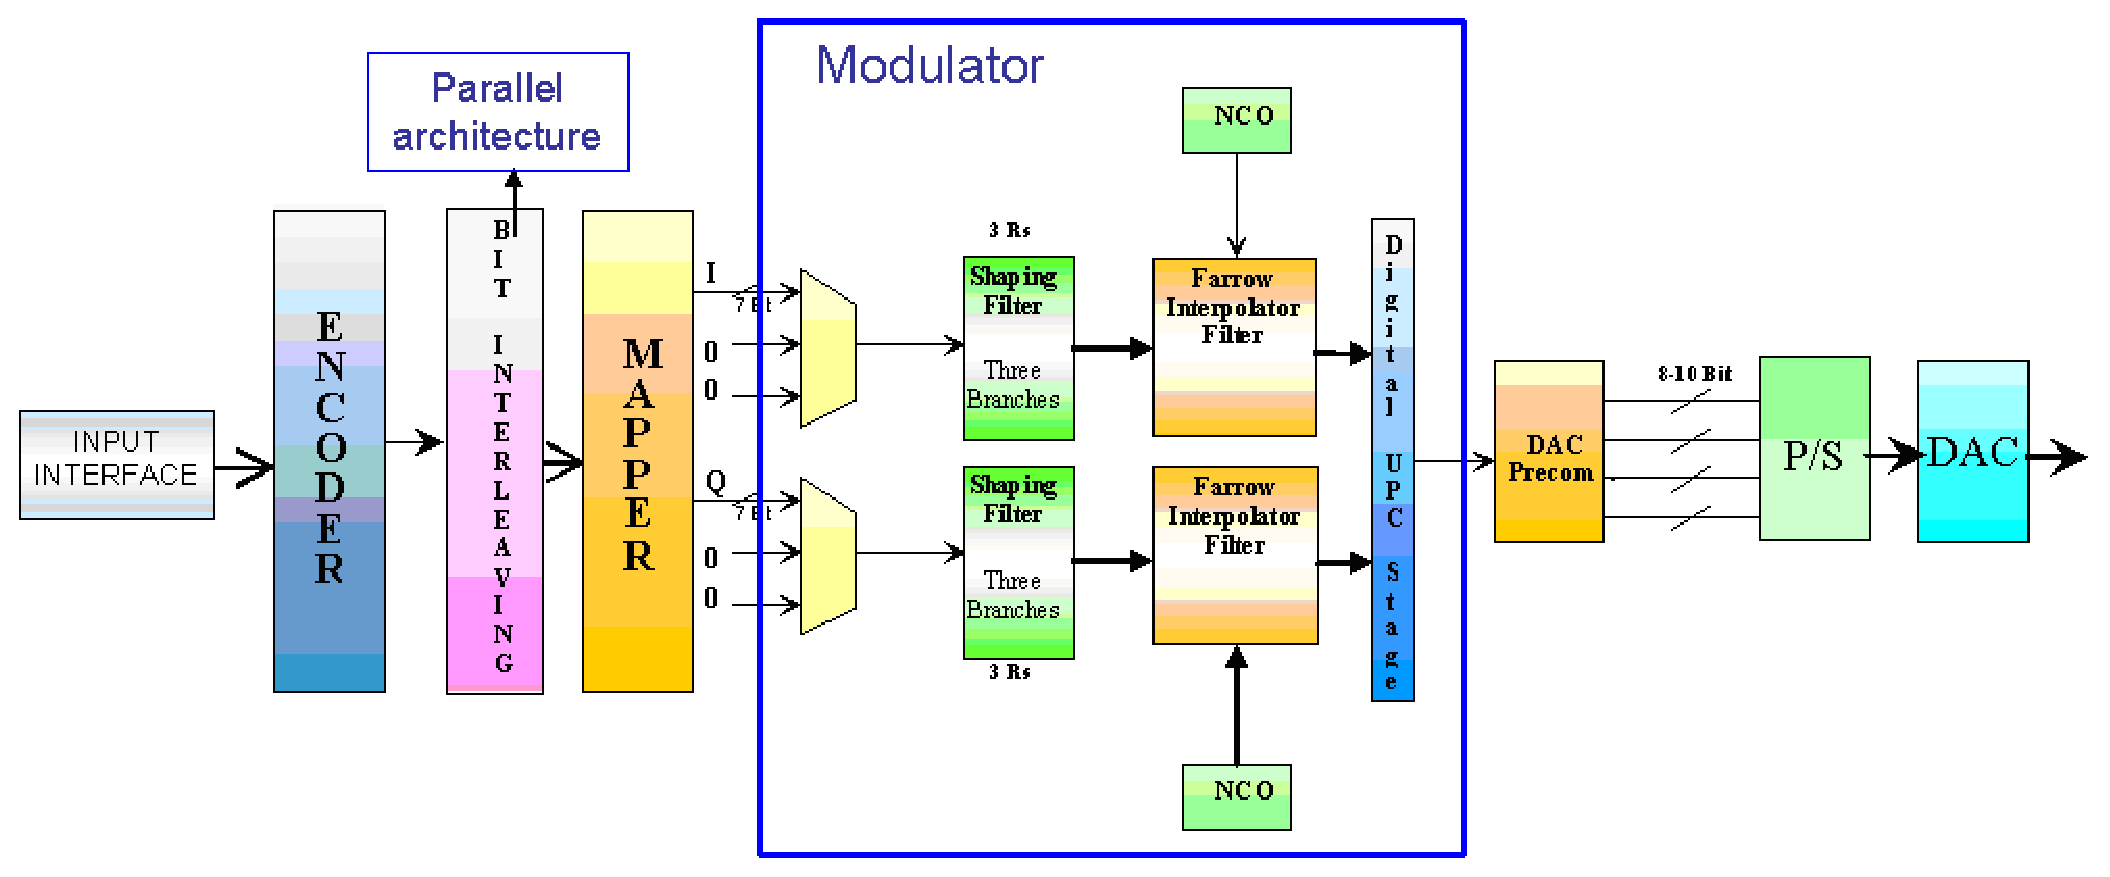
\includegraphics[scale=0.55, angle=90]{TXSection}
\caption{TX Section Architecture}
\label{fig:TXSection}
\end{figure}

\begin{description}
\item[Input Interface] This is the flexible block acquiring the source data: as many packets as required are acquired  depending on the output symbol rate, modulation and coding rate of the PLFRAME to be generated.

\item[DVB-S2 Formatter] As described in chapter \ref{ch:DVBS2Arch&Conc}, this block composes the frame. The DVB-S2 normal FEC-frame has a fixed length of 64800 bits, excluding pilot bits insertion.

\item[Base Band Header Insertion] This block inserts a fixed length Baseband Header (BBHEADER) of 10 bytes shall be inserted in front of the DATA FIELD, describing its format (the maximum efficiency loss introduced by the BBHEADER is 0,25\% for \(n\ped{ldpc}=64800\) and 1\% for \(n\ped{ldpc}=16200\), assuming that inner code rate is \(1/2\). As said in chapter 2, Data field is simply constituted by the information bits; finally, zero-bits shall be appended after this field in order to have a constant length of \(k\ped{bch}\) bits (Padding).

\item[BB Scrambling] This block is necessary since the complete BBFRAME shall be randomized. The randomization sequence shall be synchronous with the BB\-FRAME, starting from the MSB and ending after \(k\ped{bch}\) bits. The randomization is realized by adding the BBFRAME sequence (starting from MSB) to a random sequence generated by a linear shift register and initialized at the beginning of each frame. The scrambling sequence has been stored in a ROM memory; informative bits are processed in parallel by means of a standard parallelization of a linear system.

\item[Physical Layer Scrambling Block] Prior to modulation, each PLFRAME, excluding the PLHEADER, has to be randomized for energy dispersal by multiplying the \((I+ \im Q)\) samples by a complex randomization sequence \((CI+ \im CQ)\). The randomization sequence is re-initialized at the end of each PLHEADER, besides the PLFRAME duration depends on the modulation selected, thus the randomization sequence length shall be truncated to the current PLFRAME length. The scrambling code sequences are constructed by combining two real \(m\)-sequences (generated by means of two generator polynomials of degree 18) into a complex sequence. The resulting sequences thus constitute segments of a set of \emph{Gold sequences}. The physical layer scrambling has been generated by a ROM memory which is read starting from the address 0 at the beginning of each frame.

\item[Encoder Block] This functional block provides the following functions:
    \begin{itemize}
    \item 	CRC-8 (1-Byte Cyclic Redundancy Check) insertion on the incoming packets;
    \item outer (BCH) and inner (LDPC) encoding, according to the selected coding rate (see \tbref{tb:codpar});
    \item bit interleaving, when the selected modulation format is an 8PSK.
    \end{itemize}

\item[CRC-8 Encoder] This functional block is necessary only for packetized streams only.

\item[Bit Interleaving Block] The direct implementation of the Bit Interleaving suggested by Hughes Network Systems (HNS) in the ETSI standard definition strongly reduces the maximum achievable baud rate; in effect maximum baud rate is \(f\ped{ck}/\eta\), where \(f\ped{ck}\) is the operating frequency and \(\eta\) is the modulation efficiency.

    Later on an alternative parallel architecture is introduced that doesn't present this limitation.

    Our goal has been to carry out a parallel bit interleaving by means of a block that outputs one modulation signal per clock cycle in order to maximize the achievable baud rate. In this case, if \(f\ped{ck}\) [MHz] is the operating frequency, we will have a maximum achievable baud rate equal to \(f\ped{ck}\) [MBaud].

    The goal is obtained by means of a parallel architecture, which allows to read \(\eta\) consecutive bits per clock cycle belonging to different symbols; in this way, we provide one symbol per clock cycle.

\item[Mapper Block] Mapping into constellation is carried out according to the selected modulation format (Q-PSK or 8-PSK); constellations are stored in a ROM (Read Only Memory) and a 7-bit representation has been used for \(I\) and \(Q\) components.

\item[Shaping Filter] The \(I\) and \(Q\) data paths at the output of the serial to parallel block are processed by the SRRC (Squared Root Raised Cosine) filter and polyphase interpolator included on the same structure.

    This filter is used to provide the interpolation and pulse shaping of the data in order to minimize intersymbol interference. The complex valued coded symbols stream is applied at the input of this sub-unit which performs SRRC pulse shaping by a FIR filter running at rate \(3 R\ped s\) . The choice of a processing rate equal to \(3 R\ped s\) is made considering that the desired sampling frequency  \(f\ped{SA}\) is achieved by interpolating the shaped signal; as a consequence an adequate attenuation of the signal spectrum replica, centered around the interpolator input sampling frequency, is required.
%obtained at the DDPU output,
\item[Interpolator Section] In this specific case a third order Farrow Interpolator block has been used to change the rate at the output of the polyphase filter, depending on the input bit rate selected.

\item[Digital Up Conversion (UPC) Stage] This block realizes the up-conversion from the baseband frequency to the intermediate frequency.

\item[DAC Precompensation Filter] This block has been designed to compensate the signal distortion (about \(4\unit{dB}\) from DC to half the sampling frequency) introduced by the D/A conversion; in order to correct this linear distortion a FIR filter is used, just before the DAC.

    This is most for a number of reasons, e.g. the need for complex filter coefficients in case compensation were done at base-band; however, high speed operations are actually desirable: hence, a coefficient simplification is introduced to avoid multiplications and the transpose form of a FIR filter has been used; pipelining can also be used for it to further enhance speed if required.

\end{description}

\clearpage

\section{Test Objectives and Setup}

Aim of this test campaign is to verify the encoder and modulator design and its performances in terms of constellation implementation quality: this is pursued via a statistical characterization on phase and magnitude error.

All tests have been performed after synthesizing the VHDL-based design onto a Stratix II DSP Development Board, which includes an EP2S180 device. Additionally, this board provides two 14-bit D/A converters with an up to 165-Megasample per second rate and single-ended output.

In order to best evaluate the modulator performances, signal at the output of D/A converter has been routed to an ultra-broadband Vector Signal Analyzer (VSA) which also executes demodulation. The VSA is composed by the association of:

\begin{enumerate}

\item a MSO6054A 6000 series oscilloscope (\(500\unit{MHz}\) bandwidth, \(4\unit{Gsa/s}\));

\item the 89601A vector signal analyzer software, running onto a PC interconnected to the oscilloscope via an Ethernet port.

\end{enumerate}

Test setup equipments is shown in \figref{fig:TestEqu}, Stratix II FPGA hosts the VHDL-based design.

\begin{figure} \centering
\includegraphics[scale=.8]{te1}
\caption{Laboratory Test} \label{fig:TestEqu}
\end{figure}

In particular, sampling rate and IF center frequency have been designed in order to meet the requirements in presence of the HW constraints imposed by both the prototyping board and the anti-image filters available. A parallel to serial converter at the output of modulator has been added to serialize the four parallel data streams at the output of Tx section. Note that the four parallel flows are normally necessary to relax the high speed as well as the relevant criticality in the transfer of data from the TX DSP section to the DAC. The overall transmitter schematic diagram is shown in figure above.

Tx section performances have been evaluated in terms of constellation quality, furthermore, a statistical analysis of magnitude and phase errors has been computed exploiting the dedicated tool available in VSA.

The tool is based on the EVM (Error Vector Magnitude) analysis. EVM is the Root Mean Square (RMS) of the error vectors computed and expressed as a percentage of the square root of the mean power of the ideal signal. The instrument, apart from peak values, can also provide the statistically estimated standard deviation of the EVM and of the phase error.

The error vector is the magnitude of the vector, at the detected symbol location, which connects the I/Q reference-signal phasor to the I/Q measured-signal phasor, and is computed as follows (for a graphical representation refer to the phasor diagram shown below):
\begin{equation}
\mathrm{EVM}[n] = \sqrt{{I\ped{err}[n]}^2 + {Q\ped{err}[n]}^2}
\end{equation}
where the variable \(n\) indicates the discrete symbol time and obviously the error in phase is \(I\ped{err} = I\ped{Ref}-I\ped{Meas}\), that is, the reference \(I\) component is subtracted to the measured component.
In a similar way the component of error in quadrature can be measured as follow: \(Q\ped{err} = Q\ped{Ref}-Q\ped{Meas}\).

\begin{figure} \centering
\includegraphics[scale=.8]{EVMAGN}
\caption{Error vector magnitude computation} \label{fig:EVMAGN}
\end{figure}

In addition, magnitude error and phase error (computed as described in \figref{fig:MAGNPHASE}) vs time diagram (expressed in symbols) have been plotted to better evaluate constellation quality.

\begin{figure} \centering
\includegraphics[scale=.8]{MAGNPHASE}
\caption{Magnitude and phase error computation} \label{fig:MAGNPHASE}
\end{figure}

\clearpage

\section{Test Results}

In this preliminary test campaign, some measurements on the developed DVB-S2 TX section have been performed. For both \(2 \unit{MBaud}\) and \(30 \unit{MBaud}\) symbol rates, demodulated signal constellations have been plotted.

From a statistical point of view, modulator performance have been evaluated computing phase and magnitude error in the way indicated before.

From results of these preliminary test, degradation due to imperfect image rejection and DAC distortion is clear.

\subsection{2 MBaud --- 16 APSK}

In this test, signal constellation demodulated by VSA has been visually and qualitatively analyzed. In addition, phase and magnitude error have been plotted and quantified via statistical measurements to better analyze the modulation quality.

\begin{figure} \centering
\includegraphics[scale=1.2]{2MBaud16APSK2}
\caption{2MBaud 16 APSK constellation} \label{fig:16PSK2MBaud}
\end{figure}

The statistical analysis of errors leads to the following results:

\begin{center}\begin{tabular}{||p{4.22cm}||p{4.03cm}||}
\hline
 \multicolumn{1}{|p{4.22cm}|}{\centering EVM} &  \multicolumn{1}{p{4.03cm}|}{\centering 2\%} \\
 \multicolumn{1}{|p{4.22cm}|}{\centering Magnitude Error} &  \multicolumn{1}{p{4.03cm}|}{\centering 0,9\%} \\
 \multicolumn{1}{|p{4.22cm}|}{\centering Phase Error} &  \multicolumn{1}{p{4.03cm}|}{\centering 3 deg} \\
\hline
\end{tabular}\end{center}
A very limited degradation with respect to the ideal constellation is actually evident.
%\begin{figure} \centering
%\includegraphics[scale=0.8]{IQerr}
%\caption{\(I\)-\(Q\) Magnitude Error (16-APSK --- 2 MBaud)}
%\end{figure}

%\begin{figure} \centering
%\includegraphics[scale=0.8]{IQPHA16APSK}
%\caption{\(I\)-\(Q\) Phase Error (16-APSK --- 2 MBaud)}
%\end{figure}

\begin{figure} \centering
\subfloat[Signal Spectrum]{
\includegraphics[scale=.8]{Spectrum16APSK2MB}
} \qquad
\subfloat[Replica Distance]{
\includegraphics[scale=.8]{SpectrRepl2MB}
}
\caption{\(2 \unit{MBaud}\) 16-APSK Signal spectra} \label{fig:SigReplica}
\end{figure}

\clearpage

\subsection{30 MBaud --- 8 PSK}

In this test, degradation of modulator performances due to the absence of a DAC pre-compensation filter is clear. In following figures a less scattered plot with pre-compensation filter can be seen.

\begin{figure} \centering
\subfloat[Signal constellation quality in presence of DAC compensation]{
\includegraphics[scale=.8]{8PSKConst}
} \qquad
\subfloat[Signal constellation quality in absence of DAC compensation]{
\includegraphics[scale=.8]{8PSKConstNDAC} \label{fig:noDAC}
} %\qquad
%\subfloat[Signal constellation quality in presence of DAC compensation]{
%\includegraphics[scale=.8]{8PSKdac}
%} \qquad
%\subfloat[Signal constellation quality in absence of DAC compensation]{
%\includegraphics[scale=.8]{8PSKnodac}
%}
\caption{\(30 \unit{MBaud}\) 8-PSK Scatter Plots} \label{fig:8PSK30MBaud}
\end{figure}

Signal spectra comparison in \figref{fig:SpectrComp} shows the distortion introduced by the DAC: the blue curve, as a matter of fact, is the no-precompensated signal spectrum, which results in a very scattered constellation (\figref{fig:noDAC}); the yellow one, representing the signal spectrum of the same signal processed by the precompensation filter, results in a better scatter plot.

\begin{figure} \centering
\includegraphics[scale=1.3]{DACvsNDAC}
\caption{Spectra comparison between the spectrum of the signal precompensated (yellow one) and that of the signal non-precompensated (blue one)} \label{fig:SpectrComp}
\end{figure}


The statistical analysis of errors leads to the following results:
\begin{center}\begin{tabular}{||p{3.13cm}||p{4.91cm}p{4.78cm}||}
\hline
 \multicolumn{1}{|p{3.13cm}|}{\centering} &  \multicolumn{1}{p{4.91cm}}{\centering Without pre-compensation filter} &  \multicolumn{1}{p{4.78cm}|}{\centering With pre-compensation filter} \\
\hline
 \multicolumn{1}{|p{3.13cm}|}{\centering EVM} &  \multicolumn{1}{p{4.91cm}}{\centering 9\%} &  \multicolumn{1}{p{4.78cm}|}{\centering 4\%} \\
 \multicolumn{1}{|p{3.13cm}|}{\centering Magnitude Error} &  \multicolumn{1}{p{4.91cm}}{\centering 6\%} &  \multicolumn{1}{p{4.78cm}|}{\centering 2\%} \\
 \multicolumn{1}{|p{3.13cm}|}{\centering Phase Error} &  \multicolumn{1}{p{4.91cm}}{\centering 3 deg} &  \multicolumn{1}{p{4.78cm}|}{\centering 1,5 deg} \\
\hline
\end{tabular}\end{center}



%\begin{figure} \centering
%\includegraphics[scale=.8]{IQMagn8PSK}
%\caption{I-Q Magnitude Error (30 MBaud 8-PSK)}
%\end{figure}

%\begin{figure} \centering
%\includegraphics[scale=.8]{IQPha8PSK}
%\caption{I-Q Phase Error (30 MBaud 8-PSK)}
%\end{figure}

\clearpage

\subsection{30 MBaud --- 16 APSK}

In this test, signal constellation demodulated by VSA has been visually and qualitatively analyzed. In addition, phase and magnitude error have been plotted and quantified via statistical measurements to better analyze the modulation quality.


\begin{figure} \centering
\subfloat[Scatter]{
\includegraphics[scale=.8]{16APSKSca1}
} \qquad
\subfloat[Scatter]{
\includegraphics[scale=.8]{16APSKSca2}
} \caption{\(30 \unit{MBaud}\) 16-APSK Scatter Plots} \label{fig:16APSK30MBaud}
\end{figure}

The statistical analysis of errors leads to the following results:
\begin{center}\begin{tabular}{||p{4.22cm}||p{4.03cm}||}
\hline
 \multicolumn{1}{|p{4.22cm}|}{\centering EVM} &  \multicolumn{1}{p{4.03cm}|}{\centering 3\%} \\
 \multicolumn{1}{|p{4.22cm}|}{\centering Magnitude Error} &  \multicolumn{1}{p{4.03cm}|}{\centering 1,5\%} \\
 \multicolumn{1}{|p{4.22cm}|}{\centering Phase Error} &  \multicolumn{1}{p{4.03cm}|}{\centering 2 deg} \\
\hline
\end{tabular}\end{center}


%\begin{figure} \centering
%\includegraphics[scale=.8]{IQMagn1630MB}
%\caption{I-Q Magnitude Error (30 MBaud 16-APSK)}
%\end{figure}

%\begin{figure} \centering
%\includegraphics[scale=.8]{IQPha1630MB}
%\caption{I-Q Phase Error (30 MBaud} 16-APSK)}
%\end{figure}

\clearpage

\section{64-APSK Modulator}

The modulator tested by TAS can also provide modulations of higher order with respect to DVB-S2 (e.g. MHOMS modulation schemes). Figure shows a progressive expansion of time-scale representation for a 64-APSK modulation scheme, being this the most innovative modulation, and the four signal envelope level either(points lie on 4 concentric circumferences, that is, each radius represents the amplitude of each level provided).


\begin{figure} \centering
\subfloat[]{
\includegraphics[scale=.8]{64APSK1}
} \qquad
\subfloat[]{
\includegraphics[scale=.8]{64APSK2}
} \qquad
\subfloat[]{
\includegraphics[scale=.8]{64APSK3}
} \qquad
\subfloat[]{
\includegraphics[scale=.8]{64APSK4}
}
\caption{64-APSK Signal} \label{fig:64APSKwvform}
\end{figure}

\chapter{Conclusions} \label{ch:Conclusions}

In this thesis we have dealt with a digital communications TX section which can provide a reliable information transmission via satellite while complying with the challenging requirements on performance imposed by DVB-S2 standard.

My most working contributions to the overall project of the DVB-S2 TX section developed by TAS-I have been focused specifically on
\begin{itemize}
\item study of the theory underlying the BCH code: Galois fields and cyclic codes theory in order to have the theoretical basis to understand the DVB-S2 code structure and analyze algorithms related to;
\item theoretical analysis of DVB-S2 BCH code structure from which we have reach the conclusion that the DVB-S2 outer code (BCH) must be \emph{primitive} and \emph{shortened};
\item study of the BCH encoding procedures and algorithms and its related (serial) architectures;
\item modelling and design of a parallel BCH encoder with an high degree of parallelism in order to best match the TX Section (developed by TAS) speed requirements;
\item development of a Berlekamp-Massey software decoder in order give a proof of the error correction capacity of the code (encoder); to this purpose we have defined specifical routines aimed to compute arithmetic tables useful in decoding and error detection computations;
\item development of a software package (C/C++) in order to verify the functioning of architectures envisaged and give support to VLSI designers in validation of the correspondent VHDL model;
\end{itemize}

Concerning to the DVB-S2 architecture and overall TX section and thanks to the contribution of the TAS-I Algorithm \& Architectures team, this thesis has dealt with:
\begin{itemize}
\item identification of the strategic importance of satellite communications in some application scenarios such as Multimedia, Earth observation, radio-localization and navigation, \emph{etc.};
\item review of novel techniques aimed at obtaining top performance by handling modulation and coding schemes jointly;
\item assessment of the features of ACM techniques, which allow to better utilization of resources onboard while ensuring an high QoS (Quality of Service);
\item design of the DVB-S2 Modem architecture and blocks focusing on concatenated coding (BCH-LDPC) and modulation schemes;
\item qualitative description of LDPC encoding/decoding algorithms, and on the latter we have highlighted the importance of the BCH code to counteract against error floors affecting LDPC \emph{iterative decodings};
\item BCH encoding procedures and algorithms and its related (serial) architectures;
\item modelling and design of a parallel encoder with an high degree of parallelism in order to best match the TX Section (developed by TAS-I) speed requirements;
\item selection between two possible (and functionally equivalent) BCH parallel architectures in order to work in ACM;
\item development of a Berlekamp-Massey software decoder in order give a proof of the error correction capacity of the code (encoder); to this purpose we have defined specifical routines aimed to compute arithmetic tables useful in decoding and error detection computations;
\item development of a software package (C/C++) in order to verify the functioning of architectures envisaged and give support to VLSI designers in validation of the correspondent VHDL model;
\item participation to a preliminary laboratory test and validation of the TAS-I developed DVB-S2 TX section  .
\end{itemize}
%Before the equipment production, the work in progress will be devoted to
%\begin{itemize}
%\item evaluate and thus analyze BER curves by simulations
%\item measurement and BER analysis by a commercial BER meter
%\item compare BERs obtained by the BER meter with those theoretically expected
%\end{itemize}


\appendix
\include{basic}
\include{bibliografy}
\end{document} 